\chapter{Heavy Quark and Chiral Symmetries}

\epigraph{The difficulties in quantum theory are of two kinds. I might call them Class One difficulties and Class Two difficulties. Class One difficulties are the difficulties I have already mentioned: How can one form a consistent picture behind the rules for the present quantum theory? These Class One difficulties do not really worry the physicist. If the physicist knows how to calculate results and compare them with experiment, he is quite happy if the results agree with his experiments, and that is all he needs. It is only the philosopher, wanting to have a satisfying description of nature, who is bothered by Class One difficulties. There are, in addition to the Class One difficulties, the Class Two difficulties, which stem from the fact that the present laws of quantum theory are not always adequate to give any results.}{(Paul A. M. Dirac, \emph{The Evolution of the Physicist's Picture of Nature})}

%It is only the philosopher, wanting to have a satisfying description of nature, who is bothered by Class One difficulties.

In this chapter I introduce the theoretical framework in which the calculations that will be described in the next chapter have been performed. I first review the fundamentals of QCD and the reasons that lead to the use of effective theories. After a general introduction to them, I focus on the effective theories that are relevant for the research work presented in this thesis: the heavy quark effective theory and the chiral perturbation theory. Finally I introduce the chiral heavy quark theory, in which it is possible to study strong interactions of heavy hadrons with light pseudoscalar mesons.

\section{Elements of Quantum Chromodynamics}
\label{sec:chromodynamics_elements}

Quantum ChromoDynamics (QCD) is the theory of strong interactions, that is the interactions which bind together the constituents of the hadrons. This theory originated in the 60's from the work of Gell-Mann, who used group theoretical ideas to classify hadrons in almost degenerate multiplets (the so-called \emph{Eightfold Way}) and since the 70's is the most accredited theory describing hadronic physics. The fundamental particles of this theory are the \emph{quarks}, which come in six \emph{flavours} and can be organized in three \emph{families} or \emph{generations} of two flavours each (table \ref{tab:quark_masses}).

\begin{table}
  \centering
  \begin{tabular}{c c c c c c}
    \toprule
    \multicolumn{2}{c}{First Generation} & \multicolumn{2}{c}{Second Generation} & \multicolumn{2}{c}{Third Generation} \\
    Flavour & Mass [MeV] & Flavour & Mass [MeV] & Flavour & Mass [MeV] \\
    \midrule
    $d$ & $4.7$ & $s$ & $96$ & $b$ & $4 \ 180$ \\
    $u$ & $2.2$ & $c$ & $1 \ 280$ & $t$ & $173 \ 100$ \\
    \bottomrule
  \end{tabular}
  \label{tab:quark_masses}
  \caption{Quark generations and masses \cite{Patrignani:2016xqp}.}
\end{table}

QCD is gauge field theory, i.e. a theory described by a Lagrangian density invariant under local transformations of a (gauge) symmetry group. In the case of QCD, this group is $SU(3)$, that is the group of unitary unimodular $3 \times 3$ matrices. Since $SU(3)$ is a non-Abelian group, QCD belongs to the class of Yang-Mills theories. In the following this group will be denoted as $SU(3)_C$, with the subscript $C$ meaning \emph{colour}, the quantum number of quarks.

The transformations of a finite dimensional representation of $SU(3)$ have the form (sum over repeated indices is understood)
\begin{equation}
  U(\theta) = e^{- i \theta^a T^a}
\end{equation}
where the matrices $T^a$ are the eight generators of $SU(3)$ (which depend on the representation) while the scalars $\theta^a$ are the parameters of the transformation. The generators satisfy the commutation relation
\begin{equation}
  \left[ T^a , T^b \right] = i f^{a b c} T^c ,
\end{equation}
with $f^{a b c}$ structure constants of $SU(3)$. In the fundamental representation holds
\begin{equation}
  T^a = \lambda^a / 2 ,
\end{equation}
where $\lambda^a$ are the Gell-Mann matrices, while in the adjoint
\begin{equation}
  (T^a)_{b c} = -i f^{a b c} . 
\end{equation}
Moreover, the generators always satisfy the relation
\begin{equation}
  \tr{\left[ T^a T^b \right]} = C(r) \; \delta^{a b} ,
\end{equation}
where $C(r)$ is a constant that depends on the representation $r$. In particular, for the fundamental representation one has $C(r)=1/2$, while in the adjoint $C(r)=3$.

Quarks belong to the fundamental representation of $SU(3)$. Therefore they can be written as triplets, the components of which are conventionally labelled red, green and blue. Their transformation law under a finite, global $SU(3)_C$ transformation is $ q_a \mapsto U_{a b}(\theta) q_b$.

The free Dirac Lagrangian
\begin{equation}
  \symcal{L}_\text{Dirac} = \adj{q} \left( i \slashed{\partial} - m \right) q
  \label{eq:free_dirac_lagrangian}
\end{equation}
is invariant under such transformations but not under local ones, i.e. transformations in which the parameters depend on coordinates. However, \emph{if we manage to substitute the partial derivative in \eqref{eq:free_dirac_lagrangian} with an operator which transforms in a covariant manner, then the Dirac Lagrangian would become automatically invariant under local transformations}. Such an operator is called \emph{covariant derivative} and is defined in the following way
\begin{equation}
  D_\mu q = \left( \partial_\mu - i g \symbf{A}_\mu \right) q ,
  \label{eq:covariant_derivative}
\end{equation}
where $\symbf{A}_\mu$ are gauge fields with transformation law
\begin{equation}
  \symbf{A}_\mu \mapsto U \symbf{A}_\mu U^{-1} + \frac{i}{g} U \partial_\mu U^{-1} 
\end{equation}
and $g$ is the coupling constant of the theory. 

$\symbf{A}_\mu$ can be decomposed with respect to the generators $\symbf{A}_\mu = A^a_\mu T^a$.  After quantization, the quanta of the vector fields $A^a_\mu$ are called gluons. The variation of the gluon field with respect to a local infinitesimal transformation is
\begin{equation}
  \delta A^a_\mu = f^{a b c} \theta^b A^c_\mu - \frac{1}{g} \partial_\mu \theta^a ,
\end{equation}
which shows that it transforms according the adjoint representation of $SU(3)$.

After the use of the covariant derivative in place of the partial derivative in \eqref{eq:free_dirac_lagrangian}, a new Lagrangian density is obtained, consisting of the kinetic term for quarks plus a term describing quark-gluon interactions. 

However, at this point, the gauge field is a background field with no dynamics. In order to account for the latter, the Lagrangian needs to be supplemented by a pure-gauge term. For this purpose, in analogy with Quantum ElectroDynamics (QED), a field strength tensor $\symbf{G}_{\mu \nu}$ is introduced through the relation
\begin{equation}
  \left[ i D_\mu , i D_\nu \right] q = i g \symbf{G}_{\mu \nu} q = i g G^a_{\mu \nu} T^a q ,
\end{equation}
finding that
\begin{equation}
  G^a_{\mu \nu} = \partial_\mu A^a_\nu - \partial_\nu A^a_\mu + g f^{a b c} A^b_\mu A^c_\nu .
\end{equation}

$\symbf{G}_{\mu \nu}$ is covariant, i.e. it transforms with law $\symbf{G}_{\mu \nu} \mapsto U \symbf{G}_{\mu \nu} U^{-1}$, as well as every product of tensors $\symbf{G}_{\mu \nu} \cdots \symbf{G}_{\alpha \beta}$. Hence, the traces in colour space of these objects are gauge invariant. The simplest Lorentz and parity invariant term of this type is $\tr{\left[ \symbf{G}_{\mu \nu} \symbf{G}^{\mu \nu} \right]}$. Therefore, a natural choice for the pure gauge Lagrangian is
\begin{equation}
  \symcal{L}_\text{gauge} = - \frac{1}{2} \tr{\left[ \symbf{G}_{\mu \nu} \symbf{G}^{\mu \nu} \right]} = - \frac{1}{4} G^a_{\mu \nu} G^{a \mu \nu},
  \label{eq:pure_gauge_lagrangian}
\end{equation}
where the prefactor is such that, in the Abelian case, \eqref{eq:pure_gauge_lagrangian} reduces to the free Maxwell Lagrangian. Finally, we can write
\begin{equation}
  \symcal{L}_\text{QCD} = \sum_{\substack{f = d, u, s, \\ c, b, t}} \adj{q}_f \left( i \slashed{D} - m_f \right) q_f - \frac{1}{4} G^a_{\mu \nu} G^{a \mu \nu} .
\end{equation}

Once the Lagrangian is known, the generating functional of the theory can be used to calculate perturbatively the $n$-point correlation functions, from which, using the LSZ reduction formula, it is finally possible to calculate the scattering matrix elements.

This procedure has been very successful for the electrodynamics and for the unified theory of electroweak interactions, however, in the case of QCD it has to be applied with care. Indeed, as for all field theories, the coupling constant of QCD is a \emph{running} quantity, i.e. it depends on the scale at which it is measured. At odds with what happens with QED, the coupling constant is small in correspondence of large momentum scales or, analogously, at short distances. This phenomenon is called \emph{asymptotic freedom} and implies that in the ultraviolet limit the quarks propagate almost freely. 

However, for small momenta, the coupling constant is large, so that quarks are confined inside hadrons, a phenomenon known as \emph{colour confinement}. This is why only colour singlet states are experimentally observed.

Therefore, QCD has a phase diagram which shows at least two phases: one in which the Degrees of Freedom (DoF's) are the quarks and gluons and one in which they are the hadrons. These are the only true relativistic bound states known (for example, in nucleons the binding energy accounts for more than $99\%$ of the mass) and, at the present, there is no analytic tool to describe such states in terms of their fundamental constituents. However, it is still possible to use field theoretical techniques to attempt an approximate description of strong interactions at low energies through effective field theories.

\section{Some General Remarks About Effective Theories}
\label{sec:et_general_remarks}

Effective theories give an approximate description of phenomenological observations conducted in certain conditions or regimes. In this thesis, the focus is on low-energy effective theories, which fall under two categories: decoupling or non-decoupling \cite{Ecker:2005ny}. The effective theory for strong interactions which will be introduced in this chapter and used in the following, make use and combine aspects of both.

\subsection{Decoupling Effective Theories}

In decoupling effective theories, below some energy scale $\Lambda$, the DoF's of the (the sector of) the fundamental theory which one would like to describe remain the same, except that particles with mass $M \gg \Lambda$ are integrated out. 

This fact can be stated more formally saying that, in the considered kinematic region, the $n$-point functions with heavy DoF's on external legs vanish. Such $n$-point functions can be obtained from a new generating functional $Z'$, which is obtained from the old one $Z$, by a marginalization procedure. This procedure consists in decoupling the heavy DoF's from external currents in the expression of $Z$ and integrating them out. In many cases of interest, the functional integral defining $Z$ is Gaussian with respect to the heavy DoF's and hence $Z'$ can be computed analytically. 

Let be $\phi$ the heavy DoF of the theory with equation of motion
\begin{equation}
  K_0 \phi = \chi ,
  \label{eq:phi_equation_of_motion}
\end{equation}
where $K_0$ is a linear operator and $\chi$ is a function of the other fields. It follows that (neglecting a surface term) the relevant part of the generating functional $Z'$ can be cast in the following form
\begin{equation}
  Z'_\phi = \int \! \left[ \D \phi \right] \; e^{ - \frac{i}{2} \left( \phi , K_0 \phi \right) + i \left( \chi, \phi \right)} \propto \det{\Delta_0} \exp{\left( \frac{i}{2} (\chi, \Delta_0 \chi) \right)}
\end{equation}
where $\Delta_0 = K_0^{-1}$. 

If $\det{\Delta_0}$ does not introduce quantum corrections, then the whole procedure is equivalent to using the equation of motion \eqref{eq:phi_equation_of_motion} in the Lagrangian.

Finally, $Z'_\phi$ corresponds to a non-local action and hence, in order to apply the usual perturbation theory techniques, it is necessary to perform a so-called \emph{OPE} (Operator Product Expansion) of $\Delta_0$, i.e. expanding it in a series of local operators with increasing powers of $1/M$. These terms contain the dynamics at energy scales greater than $\Lambda$ and may be treated perturbatively.

Examples of decoupling effective theories are the Fermi theory of weak interactions, the Euler-Heisenberg non-linear electrodynamics, the non-relativistic Electrodynamics and the heavy quark effective theory.

%The procedure briefly reviewed is shown in the following example. Let be 
%\begin{equation}
%  \symcal{L} ( \psi, \phi ) = \adj{\psi} \left( \slashed{\partial} - m \right) \psi + \frac{1}{2} \partial_\mu \phi \partial^\mu \phi - \frac{1}{2} M^2 \phi^2 + \phi \adj{\psi} \psi 
%\end{equation}
%where $\psi$ is a Dirac field with mass $m$ and $\phi$ a scalar field with mass $M$ much greater than the energy scale in consideration. In the beginning, the generating functional 
%\begin{equation}
%  Z[\adj{\eta}, \eta, \chi] = \int \! \left[ \D \psi \right] \left[ \D \adj{\psi} \right] \left[ \D \phi \right] \; \exp \left( i \int \! \D^4 \! x \; \symcal{L} \left(\psi, \phi \right) + \adj{\eta} \psi + \adj{\psi}\eta + \chi \phi \right) 
%\end{equation}
%depends on the external current $\chi$, which is coupled to $\phi$. Passing from the original theory to the effective one, in order to integrate $\phi$ in $Z$, $\chi$ is set to zero.
%
%The relevant part of the partition function is
%\begin{equation}
%  Z_\phi [J] = \int \! \left[ \D \! \phi \right] \; \exp \left( i \int \! \D^4 \! x \; \frac{1}{2} \partial_\mu \phi \partial^\mu \phi - \frac{1}{2} M^2 \phi + \phi \adj{\psi} \psi \right) .
%\end{equation}
%
%<------------->
%
%Let $\phi_s$ be a solution of the equation of motion of the free field
%\begin{equation}
%  \left. \frac{\delta S_0}{\delta \phi} \right\vert_{\phi_s} = 0 ,
%\end{equation}
%then, the action $S_0$ can be written as a power series in $\Delta \phi = \phi - \phi_s$ around $\phi_s$
%\begin{equation}
%  S_0 [\phi_s + \Delta \phi] = S_0 [\phi_s] + \frac{1}{2} ( \Delta \phi, \left. \frac{\delta^2 S_0}{\delta \phi^2} \right\vert_{\phi_s} \Delta \phi ) + \symcal{O}(\phi^3) .
%\end{equation}
%However, the constant $S_0 [\phi_s]$ has no dynamical relevance and, since there are no auto-interaction terms, it's legit to assume that there are no terms of order $\symcal{O}(\phi^3)$, so
%\begin{equation}
%  S_0 [\phi] = \frac{1}{2} ( \Delta \phi , \left. \frac{\delta^2 S}{\delta \phi^2} \right\vert_{\phi_s} \Delta \phi) .
%\end{equation}
%
%We assume that the solutions of the Euler-Lagrange equation for the free field can be cast (neglecting a four-divergence) as the kernel of a symmetric, positive definite, linear operator $K_0$, that is 
%\begin{equation}
%  \frac{\delta S_0}{\delta \phi} = - K_0 \phi \implies \frac{\delta^2 S_0}{\delta \phi^2} = - K_0 .
%\end{equation}
%As $K_0 \phi_s = 0$, in the end we can write
%\begin{equation}
%  S_0 [\phi] = - \frac{1}{2} ( \phi , K_0 \phi ) .
%  \label{eq:quadratic_action}
%\end{equation}
%<---------------->
%Neglecting a four-divergence, the latter can be written as
%\begin{equation}
%  Z_\phi = \int \! \left[ \D \! \phi \right] \; \exp \left( - \frac{i}{2} (\phi , K_0 \phi) + i (J, \phi) \right) = \symcal{N} \det \Delta_0 \exp \left( \frac{i}{2} (J, \Delta_0 J) \right) ,
%\end{equation}
%where $K_0 = \left( \partial^2 + M^2 \right)$, $J = \adj{\psi} \psi$ and $\Delta_0 = K_0^{-1}$ is the free field propagator.
%%\begin{equation}
%%  \int \! \D^4 \! y \; K_0 (x, y) \Delta_0 (y, z) = \delta (x - z) .
%%\end{equation}
%Therefore the $n$-point functions of the effective theory can be derived from
%\begin{multline}
%  Z[\adj{\eta}, \eta] \propto \int \! \left[ \D \! \psi \right] \left[ \D \! \adj{\psi} \right] \; \exp \left( i \int \! \D^4 \! x \; \adj{\psi}(x) \left( i \slashed{\partial} - m \right) \psi(x) + \adj{\eta}(x) \psi(x) + \adj{\psi}(x) \eta(x) \right. \\ \left. + i \int \! \D^4 \! x \D^4 \! y \; \adj{\psi}(x)\psi(x) \Delta_0 (x, y) \adj{\psi}(y)\psi(y) \right) ,
%\end{multline}
%which contain a non-local action term.
%
%In this regard, an important observation is that \emph{one would have obtained the same result using the equation of motion in the action}
%\begin{equation}
%  \phi = \Delta_0 J \implies - \frac{1}{2} ( \phi , K_0 \phi ) + ( J , \phi ) = \frac{1}{2} ( J, \Delta_0 J ) .
%\end{equation}
%However, in general, if one considers a heavy DoF coupled to a gauge field, this is no more true. As a matter of fact, as long as the action can be cast as a quadratic form, the preceding considerations remain valid, but \emph{there may be contributions from the determinant of the propagator}, which is not a constant as it depends on the gauge fields. These contributions represent quantum corrections.

The most notorious example of decoupling effective theory is the Fermi theory of beta decay. In this case, the heavy DoF which decouples at low energy is the charged intermediate vector boson $W$. The relevant part of its Lagrangian is 
\begin{multline}
  \symcal{L}_W = - \frac{1}{2} \left( \partial_\mu W^-_\nu - \partial_\nu W^-_\mu \right) \left( \partial^\mu W^{+ \nu} - \partial^\nu W^{+ \mu} \right) \\ + M_W^2 W^-_\mu W^{+ \mu} + \frac{g}{2 \sqrt{2}} \left( J^-_\mu W^{+ \mu} + W^-_\mu J^{+ \mu} \right) ,
\end{multline}
with
\begin{equation}
  W^- = (W^+)^\dagger \qquad J^- = (J^+)^\dagger ,
\end{equation}
where, in the Weinberg-Glashow-Salam theory of electroweak interactions, $g$ is the coupling constant of the $SU(2)$ gauge field and, in the hadronic sector
\begin{equation}
  J^+_\mu = V_{p n} \adj{p} \gamma_\mu ( 1 - \gamma^5 ) n \qquad p = (u, c, t) \qquad n = (d, s, b) ,
\end{equation}
where $V_{p n}$ is the relevant element of the Cabibbo-Kobayashi-Maskawa matrix, while in the leptonic one
\begin{equation}
  J^+_\mu = \adj{l} \gamma_\mu ( 1 - \gamma^5 ) \nu_l \qquad l = (e, \mu, \tau) . 
\end{equation}

Independently of the nature of the current, the equation of motion for $W$ is 
\begin{equation}
  - ( \partial^2 + M^2_W ) W^+_\mu + \partial_\mu ( \partial_\nu W^{+ \nu} ) = \frac{g}{2 \sqrt{2}} J^+_\mu
\end{equation}
and hence, formally
\begin{equation}
  W^+_\mu = \frac{g}{2 \sqrt{2}} \Delta\indices{_\mu^\nu} J^+_\nu ,
\end{equation}
where the propagator $\Delta$ is the inverse of
\begin{equation}
  K^{\mu \nu}(x, y) = \delta(x - y) \left( - \left( \partial^2 + M_W^2 \right) g^{\mu \nu} + \partial^\mu \partial^\nu \right) ,
\end{equation}
i.e. the propagator for a massive vector field. In the momentum space the latter is
\begin{equation}
  \Delta_{\mu \nu}(k) = \frac{g_{\mu \nu} - \frac{k_\mu k_\nu}{M^2_W}}{k^2 - M^2_W} .
\end{equation}

Finally, interactions between charged current in the effective theory are described by the non-local action
\begin{equation}
  S_\text{NL} = \frac{g^2}{8} \int \! \D^4 \! x \D^4 \! y \; J^{- \mu}(x) \Delta_{\mu \nu}(x, y) J^{+ \nu}(y) .
\end{equation}
The propagator can be expanded in a series of powers of $k^2/M^2_W$
\begin{equation}
  \Delta_{\mu \nu}(k) = - \frac{1}{M^2_W} g_{\mu \nu} + \symcal{O}\left( \frac{k^2}{M^2_W} \right)
\end{equation}
and to the leading order the interaction term of the effective Lagrangian is
\begin{equation}
  \symcal{L}_\text{I} = - \frac{g^2}{8 M^2_W} J^-_\mu J^{+ \mu} ,
\end{equation}
which correspond to the current-current or point interactions of the Fermi theory. The Fermi constant $G_F=1.16632 \; 10^{-5} \ \text{GeV}^{-2}$ can be expressed in terms of the coupling $g$ through the relation 
\begin{equation}
  \frac{g^2}{8M_W^2}=\frac{G_F}{\sqrt{2}} .
\end{equation}

For the sake of this discussion, there are other two points worth noting. The first is that no new particles are generated in the transition from the fundamental to the effective level, indeed the heavy ones disappear from the theory. The second is that the coupling constants appearing in the effective Lagrangian can be calculated from the original theory through an analytic procedure.

\subsection{Non-decoupling Effective Theories} 

In this case, the original theory is subjected to a phase transition at energies lower than $\Lambda$ and its DoF's are not the fundamental fields but (possibly relativistic) bound states, which is not know how to describe in terms of their fundamental constituents. Non-decoupling effective theories are built thanks to a theorem stated by Weinberg (but never proved \cite{Weinberg:1978kz})
\begin{quote}
  [...] Quantum field theory itself has no content beyond analyticity, unitarity, cluster decomposition, and symmetry. This can be put more precisely in the context of perturbation theory: if one writes down the most general possible Lagrangian, including \emph{all} terms consistent with assumed symmetry principles, and then calculates matrix elements with this Lagrangian to any given order of perturbation theory, the result will simply be the most general possible $S$-matrix consistent with analyticity, perturbative unitarity, cluster decomposition and the assumed symmetry principles.
\end{quote}

One wants to \emph{model} bound states using effective fields, with ad-hoc internal DoF's and transformation properties, and describe their interactions in the framework of local quantum field theory, but does not know the Lagrangian for such effective fields. However, Weinberg's theorem guarantees that the most general Lagrangian will reproduce the most general scattering matrix consistent with the assumed symmetry principles. Therefore we can construct such a Lagrangian by exhaustion, including all allowed terms. The result will contain (possibly numerous) coupling constants, referred in the literature as Low Energy Constants (LEC's), which have to be deduced experimentally or calculated in some other way (e.g. using numerical lattice methods).

\section{Heavy Quark Effective Theory}
The Heavy Quark Effective Theory (HQET) describes strong interactions of heavy quarks, typically within hadrons, at energy scales much lower than their mass (for a review see \cite{Neubert:1993mb}). A quark with mass $m_Q$ is said to be a heavy quark if $m_Q \gg \Lambda_\text{QCD}$, where $\Lambda_\text{QCD}$ is the scale parameter appearing in the formula of the running of the strong coupling
\begin{equation}
  \alpha_S \left( q^2 \right) = \frac{12 \pi}{\left( 33 - 2 n_f \right) \ln \left( \frac{q^2}{\Lambda_\text{QCD}^2} \right)} ,
\end{equation}
where $n_f$ is the number of flavours and $q$ is the momentum scale. At large distances (small $q^2$) the coupling becomes large, leading to the confinement of quarks and gluons. Therefore the typical hadronic radius $R_\text{had} \approx 1 \ \text{fm}$ is of the order of $1 / \Lambda_\text{QCD}$, which means $\Lambda_\text{QCD} \approx 200 \ \text{MeV}$. Hence, the heavy quarks are $c$, $b$ and $t$. However, $t$ decays too quickly to form bound states. Conversely the light quarks are $d$, $u$ and $s$.

The HQET is obtained from QCD in the limit in which the mass of the heavy quarks tends to infinity and, at the same time, their velocity is kept fixed. This limit applies to systems containing a heavy quark interacting with other light quarks by exchanging soft gluons ($E \lessapprox \Lambda_{QCD}$). In this case, its momentum fluctuates by an amount of the order of $\Lambda_\text{QCD}$ and hence its velocity by $\Lambda_\text{QCD}/m_Q$, a quantity which vanishes in the limit $m_Q \to \infty$. Therefore, in such systems the velocity of the heavy quark is no more a DoF and becomes a conserved quantity.

The Light Degrees of Freedom (LDoF's) of such systems (light quarks and gluons) experience only the static colour field of the heavy quark and are blind to its flavour (that is, its mass) and spin orientation. This is because they interact with the heavy quark by means of soft gluons which cannot resolve distances of the order of the Compton length of the heavy quark $\lambda_Q \approx 1/m_Q$.

The HQET is a decoupling effective theory, however, the procedure outlined in the last section requires some comments. If conservation laws forbid the decay of some heavy particles, they cannot be removed from the theory at low scales and indeed, in this scenario, they act like external sources. This is the case of HQET (moreover, if one want to describe systems containing them then there is no interest in eliminating them completely from the theory). Having the physical picture in mind, the goal is to decompose the heavy quark field $Q$ in a light component $h_v$, which will survive, and a heavy one $H_v$, which will be integrated out. 

There is a strong analogy between the HQET and the non-relativistic limit of a spin-$1/2$ particle interacting with the electromagnetic field. Lets briefly review the latter. A particle of such, with mass $m_0$ and charge $e$, is described by a Dirac spinorial field $\psi$ and its Lagrangian is
\begin{equation}
  \symcal{L}_\text{QED} = \psi^\dagger \left( i \frac{\partial}{\partial t} - e \phi - \symbf{\alpha} \cdot \left(-i \symbf{\nabla} - e \symbf{A} \right) - \beta m_0 \right) \psi ,
\end{equation}
where $(\phi, \symbf{A})$ is the electromagnetic four-potential and $(\beta, \symbf{\alpha})$ are the Dirac matrices. In order to take the non-relativistic limit, we consider a particle with four-momentum $p_\mu = m_0 \delta_{\mu 0} + k_\mu$, where $k_\mu$ is small compared to $m_0$ . It is convenient to drop out the rest-frame oscillating phase and write explicitly the antiparticle and particle bispinor components
\begin{equation}
  \psi = \exp \left( - i m_0 t \right) \begin{pmatrix} \varphi \\ \chi \end{pmatrix} .
  \label{eq:nrqed_decomposition}
\end{equation}
In terms of $\varphi$ and $\chi$, the Lagrangian becomes
\begin{multline}
  \symcal{L}_\text{QED} = \varphi^\dagger \left(i \frac{\partial}{\partial t} - e \phi \right) \varphi + \chi^\dagger \left(i \frac{\partial}{\partial t} - e \phi + 2 m_0 \right) \chi \\ - \varphi^\dagger c \symbf{\sigma} \cdot \left(-i \symbf{\nabla} - e \symbf{A} \right) \chi - \chi^\dagger c \symbf{\sigma} \cdot \left(- i \symbf{\nabla} - e \symbf{A} \right) \varphi ,
\end{multline}
from which it is apparent that $\chi$ represent a DoF with mass $2 m_0$ coupled to $\phi$ (which is massless) and thus we identify the negative energy solution with the heavy DoF that has to be removed.

The equation of motion for $\chi$ is
\begin{equation}
  \left( i \frac{\partial}{\partial t} - e \phi + 2 m_0 \right) \chi = \symbf{\sigma} \cdot \left(- i \symbf{\nabla} - e \symbf{A} \right) \varphi 
\end{equation}
and its solution can be plugged in the action to integrate out $\chi$. However, because the propagator 
\begin{equation}
  \Delta_\chi = \left( i \frac{\partial}{\partial t} - e \phi + 2 m_0 \right)^{-1} 
\end{equation}
depends on the electric potential, we expect quantum corrections to arise. Nonetheless, it turns out that $\det \Delta_\chi$ is a constant, as can be easily seen in the temporal gauge where $\phi$ vanish, and hence does not introduce additional terms in the effective action.

Finally, using the relation
\begin{equation}
  \left( \symbf{\sigma} \cdot \left( -i \symbf{\nabla} - e \symbf{A} \right) \right)^2 = \left(-i \symbf{\nabla} - e \symbf{A} \right)^2 - e \symbf{\sigma} \cdot \symbf{B} ,
\end{equation}
at order $1/m_0$, the Lagrangian becomes
\begin{equation}
  \symcal{L}_\text{Pauli} = \varphi^\dagger \left(i \frac{\partial}{\partial t} - e \phi - \frac{1}{2 m_0} \left( - i \symbf{\nabla} - e \symbf{A} \right)^2  + \frac{e}{2 m_0} \symbf{\sigma} \cdot \symbf{B} \right) \varphi
\end{equation}
and the corresponding equation of motion is the famous Pauli equation
\begin{equation}
  i \frac{\partial}{\partial t} \varphi = \left( e \phi + \frac{1}{2 m_0} \left( - i \symbf{\nabla} - e \symbf{A} \right)^2 - \frac{e}{2 m_0} \symbf{\sigma} \cdot \symbf{B} \right) \varphi .
\end{equation}
As expected, the kinetic term and the coupling with the magnetic field appear as corrections of order $1/m_0$.

In the HQET, one follows exactly the same steps in a formally covariant fashion and considers a perturbation $k_\mu$ (with $k_\mu \ll m_Q$) about the four-momentum $p_\mu = m_Q v_\mu$. The phase $-i m_Q v^\mu x_\mu$ can be isolated and the positive and negative energy contributions can be made explicit by means of the energy projectors
\begin{equation}
  \operatorname{P}_\pm = \frac{m_Q \pm \slashed{p}}{2 m_Q} = \frac{1 \pm \slashed{v}}{2} .
\end{equation}
As a matter of fact, the heavy quark field $Q$ can be written in the following way
\begin{gather}
  Q(x) = e^{-i m_Q v^\mu x_\mu} \left( h_v(x) + H_v(x) \right) , \\
  \operatorname{P}_+ h_v = h_v, \quad \operatorname{P}_- H_v = H_v .
\end{gather}
This decomposition, which is the boosted version of \eqref{eq:nrqed_decomposition}, requires some comments. The four-velocity $v$ which appear in the energy projectors is a phenomenological quantity involved in the description of a particular configuration. It is not a dynamical quantity and does \textbf{not} transform covariantly under Lorentz transformations. Its meaning in HQET is that of an index. 

Keeping this in mind, it is possible to calculate how the condition $\operatorname{P}_+ h_v = h_v$ is affected by Lorentz transformations, let $\operatorname{S}(\Lambda)$ be the action of such a transformation on bispinors
\begin{equation}
  \frac{1 + \slashed{v}}{2} h_v \mapsto \frac{1 + \slashed{v}}{2} \operatorname{S}(\Lambda) h_v = \operatorname{S}(\Lambda) \frac{1 + v_\mu \adj{\operatorname{S}}(\Lambda) \gamma^\mu \operatorname{S}}{2} h_v = \operatorname{S}(\Lambda) \frac{1 + \slashed{v}^\prime}{2} h_v , 
\end{equation}
with $v' = \Lambda^{-1} v$.

The relevant part with respect to $Q$ of the QCD Lagrangian is
\begin{equation}
  \symcal{L}_\text{QCD} = \adj{Q} \left( i \slashed{D} - m_Q \right) Q 
\end{equation}
and using the property
\begin{equation}
  \operatorname{P}_\pm \slashed{D} = \slashed{D} \operatorname{P}_\mp \pm v^\mu D_\mu ,
\end{equation}
$\symcal{L}_\text{QCD}$ can be written in terms of $h_v$ and $H_v$ in the following way
\begin{equation}
  \symcal{L}_\text{QCD} = \adj{h}_v \left. i \ v^\mu D_\mu \right. h_v - \adj{H}_v \left( \left. i \ v^\mu D_\mu \right. + 2 m_Q \right) H_v + \adj{h}_v i \slashed{D}_\perp H_v + \adj{H}_v i \slashed{D}_\perp h_v ,
\end{equation}
where
\begin{equation}
  D_\perp^\mu = D^\mu - v^\mu v^\nu D_\nu .
\end{equation}

Hence $H_v$ represents a DoF with mass $2 m_Q$ coupled to $h_v$ and will be integrated out. Its equation of motion is
\begin{equation}
  \left( \left. i \ v^\mu D_\mu \right. + 2 m_Q \right) H_v = i \slashed{D}_\perp h_v ,
\end{equation}
and the general considerations for a decoupling effective theory hold. Analogously to the non-relativistic QED case, there are no quantum corrections, as can be seen in the gauge with $v \cdot A^a = 0$.

Finally, we obtain the action
\begin{equation}
  S = \int \! \D^4 \! x \; \adj{h}_v \left. i \ v^\mu D_\mu \right. h_v + \int \! \D^4 \! x \D^4 \! y \; \adj{h}_v i \slashed{D}_\perp \frac{1}{\left. i \ v^\mu D_\mu \right. + 2 m_Q} i \slashed{D}_\perp h_v ,
\end{equation}
which contains a non-local part.

An important observation is that having eliminated the negative energy solutions from the theory, this effective theory conserves the number of heavy quarks, that is pair creation is absent. De facto, the $h_v$ operators annihilate positive energy quarks but do not create negative energy antiquarks (and vice-versa for $\adj{h}_v$). If one wants to describe processes involving heavy antiquarks, a different action should be used and it can be obtained from the previous one applying the substitution $v \mapsto - v$.

The terms of order $1 / m_Q$ of the effective Lagrangian can be written in a more familiar way using the following identity 
\begin{equation}
  \operatorname{P}_+ i \slashed{D}_\perp i \slashed{D}_\perp \operatorname{P}_+ = \operatorname{P}_+ \left( (i D_\perp)^2 + \frac{g}{2} \sigma_{\alpha \beta} G^{\alpha \beta} \right) \operatorname{P}_+ ,
\end{equation}
so that it holds
\begin{equation}
  \symcal{L} = \adj{h}_v \left. i \ v^\mu D_\mu \right. h_v + \frac{1}{2 m_Q} \adj{h}_v (i D_\perp)^2 h_v + \frac{g}{4 m_Q} \adj{h}_v \sigma_{\alpha \beta} G^{\alpha \beta} h_v + \symcal{O}\left( \frac{1}{m_Q^2} \right) .
  \label{eq:qcd_lagrangian_wo_hdof}
\end{equation}

The interpretation of the two operators appearing at order $1/m_Q$ and their analogy with the non-relatistic electrodynamics is more evident in the rest frame. Within the latter, it holds that
\begin{equation}
  \symcal{O}_\text{kin} = \frac{1}{2 m_Q} \adj{h}_v (i D_\perp)^2 h_v \mapsto - \frac{1}{2 m_Q} \adj{h}_v \Vert i \symbf{D} \Vert^2 h_v ,
\end{equation}
which is the non-Abelian generalization of the covariant kinetic energy $\Vert \symbf{p} - e \symbf{A} \Vert^2 / 2 m_Q$, so that this operator is usually referred to as the HQ kinetic energy operator. Moreover, 
\begin{equation}
  \symcal{O}_\text{mag} = \frac{g}{4 m_Q} \adj{h}_v \sigma_{\alpha \beta} G^{\alpha \beta} h_v \mapsto - \frac{g}{m_Q} \adj{h}_v \symbf{S} \cdot \symbf{B}_c h_v ,
  \label{eq:heavy_chromomagnetic_operator}
\end{equation}
which is the non-Abelian generalization of the Pauli term, where
\begin{equation}
  B^i_c = - \frac{1}{2} \varepsilon^{i j k} G^{j k} , \quad S^i = \frac{1}{2} \gamma^5 \slashed{v} \slashed{e}^i 
\end{equation}
are respectively the color-magnetic field and the boosted spin operator ($\{ e^i \}$ is a dreibein of four-vectors orthogonal to $v$). $\symcal{O}_\text{mag}$ is know as the chromo-magnetic operator.

The main point is that \textbf{at the leading order, the spin and flavour of heavy quarks are decoupled}. This can be put in a more formal statement saying that the theory exhibits a $SU(2 N_h)$ symmetry, where $N_h$ is the number of heavy flavours and means that, in the HQ limit, the spin and flavour of heavy quarks are conserved quantum numbers. The analogy with the non-relativistic electrodynamics can be stressed observing that different isotopes have the same chemistry and that, in atomic physics, hyperfine levels are nearly degenerate. 

Given an observable which contain products of the heavy quark field operators, one could, in principle, by means of the relation
\begin{equation}
  Q(x) = e^{i m_Q v^\mu x_\mu} \left( 1 + \frac{1}{\left. i \ v^\mu D_\mu \right. + 2 m_Q} i \slashed{D}_\perp \right) h_v(x)
\end{equation}
expand it to the relevant order in $1 / m_Q$. There is one caveat though, there is a residual $m_Q$ dependence hidden in the $h_v$ field, which indeed, at this moment, is the solution of the equations of motion for the Lagrangian \eqref{eq:qcd_lagrangian_wo_hdof}. For example, the vector current
\begin{equation}
  V^\mu (x) = e^{- i m_Q v^\mu x_\mu} \, \adj{q}(x) \gamma^\mu \left( 1 + \frac{i \slashed{D}_\perp}{2 m_Q} + \cdots \right) h_v (x) ,
\end{equation}
can be evaluated between a heavy meson state $M(v)$ and the vacuum
\begin{equation}
  \langle 0 \rvert V^\mu \lvert M(v) \rangle = \langle 0 \rvert \adj{q} \gamma^\mu h_v \lvert M(v) \rangle + \frac{1}{2 m_Q} \langle 0 \rvert \adj{q} \gamma^\mu i \slashed{D}_\perp h_v \lvert M(v) \rangle + \cdots .
\end{equation}
However, the second term of the RHS of the previous equation is not the leading correction in $1/m_Q$. Therefore, to make fully explicit the $m_Q$ dependence and restore the correct power counting, the HQET Lagrangian is \emph{defined} as (with $\operatorname{P}_+ h_v = h_v$)
\begin{equation}
  \symcal{L}_\text{HQET} \equiv \adj{h}_v \left. i \ v^\mu D_\mu \right. h_v
  \label{eq:hqet_lagrangian}
\end{equation}
and the terms containing higher powers of $1 / m_Q$ are treated as perturbations
\begin{equation}
  \symcal{L}_\text{power} = \frac{1}{2 m_Q} \symcal{L}_1 + \frac{1}{4 m_Q^2} \symcal{L}_2 + \cdots .
  \label{eq:hqet_power_corrections}
\end{equation}
In the HQET, the equations of motion of $h_v$ are
\begin{equation}
  \begin{cases}
    v^\mu D_\mu h_v = 0 \\
    \slashed{v} h_v = h_v
  \end{cases},
\end{equation}
which does not contain the heavy quark mass $m_Q$ (and hence neither the states created acting on the vacuum with $h_v$). Taking into account these redefinitions, the previous matrix element of the vector current becomes
\begin{multline}
  \langle 0 \rvert V^\mu \lvert M(v) \rangle_\text{QCD} = \langle 0 \rvert \adj{q} \gamma^\mu h_v \lvert M(v) \rangle_\text{HQET} + \frac{1}{2 m_Q} \langle 0 \rvert \adj{q} \gamma^\mu i \slashed{D}_\perp h_v \lvert M(v) \rangle_\text{HQET} \\ + \frac{1}{2 m_Q} \langle 0 \rvert \left( i \int \! \D^4 \! y \; \operatorname{T} \left\{ \adj{q} \gamma^\mu h_v(0) , \symcal{L}_1(y) \right\} \right) \lvert M(v) \rangle_\text{HQET} + \symcal{O} \left( \frac{1}{m_Q^2} \right) .
\end{multline}

\begin{figure}
\center
  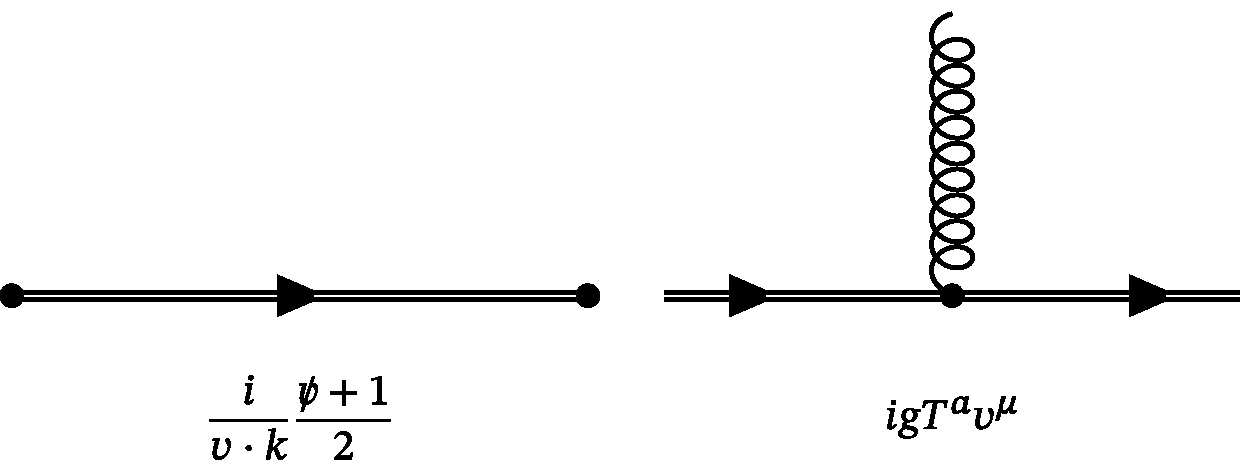
\includegraphics[width=0.8\textwidth]{figures/pdf/feynman_rules.pdf}
\caption{Feynman rules in HQET.}
\label{fig:hqet_feynman_rules}
\end{figure}

The Feynman rules of HQET (displayed in figure \ref{fig:hqet_feynman_rules}) are simpler than those of QCD and coincide with their HQ limit. For example, for the heavy quark propagator holds that
\begin{equation}
  \frac{i}{\slashed{P}_Q - m_Q} \to \frac{i}{v^\mu k_\mu} \frac{\slashed{v} + 1}{2} + \symcal{O}\left(\frac{k}{m_Q}\right) ,
\end{equation}
with $P_Q = m_Q v + k$, as $k / m_Q \to 0$. Also, the quark-gluon vertex simplifies, being evaluated between positive energy eigenstates 
\begin{equation}
  \operatorname{P}_+ \left( i g T^a \gamma^\mu \right) \operatorname{P}_+ = \operatorname{P}_+ \left( i g T^a v^\mu \right) \operatorname{P}_+ ,
\end{equation}
so that the vertex between a heavy quark and a gluon becomes simply $i g T^a v^\mu$, which does not contain gamma matrices.

It is important to observe that the HQET Lagrangian is not Lorentz invariant: under an infinitesimal transformation $\Lambda\indices{^\mu_\nu} = \delta\indices{^\mu_\nu} - i \omega\indices{^\mu_\nu}$ (acting on $h_v$ as $\operatorname{S} = \symbb{1} + \frac{i}{4} \omega_{\mu \nu} \sigma^{\mu \nu}$)
\begin{equation}
  \delta \symcal{L}_\text{HQET} = \omega\indices{^\mu_\nu} \adj{h}_v v_\mu D^\nu h_v ,
\end{equation}
indeed the selection of a particular four-velocity $v$ (i.e. a particular frame of reference, in which the heavy quark is at rest) breaks the Lorentz symmetry.

However, $\symcal{L}_\text{HQET}$ is invariant for transformations of $SU(2)$ acting on $h_v$ in the following way (for infinitesimal transformations)
\begin{equation}
  h_v \mapsto \left( 1 + i \symbf{\varepsilon} \cdot \symbf{S} \right) h_v ,
\end{equation}
which is the mathematical statement of the HQ spin symmetry of the HQET Lagrangian. Notice that these transformations preserve the positive energy condition indeed
\begin{equation}
  \operatorname{P}_+ \left( 1 + i \symbf{\varepsilon} \cdot \symbf{S} \right) h_v = \left( 1 + i \symbf{\varepsilon} \cdot \symbf{S} \right) h_v .
\end{equation}

It can be shown \cite{Mannel:1991mc} that, if one consider the full QCD Lagrangian and studies the case in which QCD interactions change the velocity of the heavy quark, in the limit $m_Q \to \infty$, the QCD Green functions involving one ingoing and one outgoing heavy quark vanish if the two velocity are different. This fact in the literature is sometimes referred to as \emph{velocity superselection rule}. Since there is no coupling among quarks with different velocities one can restore the Lorentz invariance of the HQET summing in a covariant way over the velocities (which, in this case, transform in turn covariantly). This generalization is due to Georgi \cite{Georgi:1990um} and the Lagrangian reads
\begin{equation}
  \symcal{L}_\text{HQET} = \int \! \frac{\D^3 \! v}{(2 \pi)^3} \frac{1}{2 \sqrt{\Vert \symbf{v} \Vert^2 + 1}} \; \adj{h}_v \left. i \ v^\mu D_\mu \right. h_v .
\end{equation}
It is easy to see that now $\symcal{L}_\text{HQET}$ is Lorentz-invariant, indeed for a finite transformation $\Lambda\indices{^\mu_\nu}$
\begin{multline}
  \symcal{L}_\text{HQET} = \int \! \frac{\D^4 \! v}{(2 \pi)^4} \; \delta^4 \! \left( v^2 - 1 \right) \, \theta ( v_0 ) \, \adj{h}_v \left. i \ v^\mu D_\mu \right. h_v \\ \mapsto \int \!  \frac{\D^4 \! u}{(2 \pi)^4} \; \vert \det{\Lambda} \vert \, \delta^4 \! \left( u^2 - 1 \right) \, \theta ( u_0 ) \, \adj{h}_u \left. i \ u^\mu D_\mu \right. h_u = \symcal{L}_\text{HQET} ,
\end{multline}
using the substitution $v = \Lambda u$ and taking into account that for a orthochronus Lorentz transformations holds $u_0 > 0$ and $\vert \det{\Lambda} \vert = 1$ .

\section{Spectroscopic Implications of HQET}
\label{sec:spectroscopic_implications_of_hqet}

The symmetries of HQET in the exact HQ limit provide a number of spectroscopic observable consequences:
\begin{itemize}
  \item for each hadronic state containing a heavy quark and for each flavour of the latter there is a degenerate doublet of states differing by the orientation of the heavy quark spin $\symbf{S}_Q$ and having the same full width;
  \item the sum of partial widths of strong decays between two doublets are the same for the two states of the initial doublet;
  \item the partial decay widths and mass splittings between different doublets are independent of the heavy quark flavour.
\end{itemize}

Moreover, due to the fact that, in the limit $m_Q \to \infty$, the heavy quark decouples from the LDoF, its spin $\symbf{S}_Q$ and the total angular momentum of LDoF $\symbf{S}_l$ are separately conserved. The total angular momentum of the LDoF's is the sum of the orbital angular momentum $\symbf{L}$ of the light quark with respect to the heavy quark and its spin $\symbf{S}_q$: $\symbf{S}_l = \symbf{L} + \symbf{S}_q$. However, it should be noticed that nothing prevents the existence of different states with the same values of $\symbf{S}_l$ and $\symbf{S}_Q$. These states are interpreted as \emph{radial excitations}, in analogy to non-relativistic systems (e.g. the hydrogen atom).

For the purpose of this work, from here on, I will concentrate on the heavy meson sector. Regarding the nomenclature for such particles, I will adhere to the convention of indicating the natural spin-parity series ($0^+, 1^-, 2^+, \cdots$) with an asterisk. We remember that the parity of a meson can be written as $P = (-1)^{L+1}$, having quarks and antiquarks opposite intrinsic parity. The spin of the particle will appear as a subscript, with the exception of the ground state with $S_\ell = (1/2)^-$, and the radial excitations will be indicated with a tilde.

In the ground state ($L = 0$) the quantum numbers of the LDoF's are those of the light antiquark, that is $S_\ell^P = (1/2)^-$. The corresponding doublet $(P, P^*)$ will contain a singlet state $P$ corresponding to a pseudoscalar particle with $J^P = 0^-$ and a triplet state $P^*$ corresponding to a vector one with $J^P = 1^-$. When $L =1$ two doublets can be built according to the two possible orientations of $\symbf{S}_q$. The doublet $(P_0^*, P_1)$ with $\symbf{S}_q$ antiparallel to $\symbf{L}$ will have the same angular momentum but opposite parity with respect to the ground state, that is $S_\ell = (1/2)^+$, and will contain a scalar $P_0^*$ with $J^P = 0^+$ and a pseudovector $P^\prime_1$ with $J^P = 1^+$. The other doublet $(P_1 , P_2^*)$, with $S_\ell^P = (3/2)^+$, will contain a axial particle $P_1$ with $J^P = 1^+$ and a tensor one $P_2^*$ with $J^P = 2^+$. In this way, doublets corresponding to higher values of $L$ can be analogously defined.

Let us consider the implications for the masses of these states. The ground state doublet is experimentally confirmed to be nearly degenerate both in the charm and beauty sector, with and without strangeness (within few percentage points of the mass of the state). Moreover, being the small mass splitting a relativistic correction of order $1/m_Q$, one can predict that $m^2_{D^*} - m^2_D \approx m^2_{B^*} - m^2_B$, which is also found to be true. For the same reason, one expects this relation to be true in the case of states with strangeness $m^2_{D_s^*} - m^2_{D_s} \approx m^2_{B_s^*} - m^2_{B_s}$. However, in principle, this quantity is not the same in the two cases, because the quantum numbers of the LDoF's are different. Nonetheless, the data shows that these are very similar and therefore it can be deduced that hyperfine corrections are approximately independent of the light quark flavour.

\section{Covariant Representation of Heavy Mesons}

As seen in section \ref{sec:et_general_remarks}, in non-decoupling effective theories fields with desired properties are introduced. These effective fields must belong to some representations of the symmetry group of the more fundamental theory in exam. However, these representations are in principle reducible and thus the effective fields can be decomposed in linear combinations of fields belonging to irreducible representations. Therefore, in general, effective fields represent multiplets of particles.

This is precisely the case of heavy mesons doublets. Because $\symbf{S}_Q$ and $\symbf{S}_l$ are separately conserved, as predicted by the HQET, the effective field $M$ must belong to the tensor product of the representations of $SO(3,1)$ to which belong the heavy quark and the LDoF's, i.e. the representation $ 2 \otimes \left( 2 \times S_\ell + 1 \right) =  2 \times S_\ell \oplus \left( 2 \times S_\ell + 2 \right)$.
Moreover, it must have the right parity, it must have one light and one heavy flavour indices and it must belong to the trivial representation of the $SU(3)_C$ group (because observable states are colour singlets).

% FIXME: riformulare 
%Finally, as another consequence of the HQET, there must be a frame of reference in which the heavy quark is at rest: the heavy meson effective field $M$ is built to have this property, i.e. in such a way that exist a meson energy projector $\operatorname{P}$ such that $\operatorname{P} M = M$. The frame of reference in which the meson is at rest is parametrized in the frame of reference of the laboratory by a four-velocity $v$.

Given a field $A_l$ with the quantum numbers of the LDoF's and a positive energy bispinor $\psi_h$ with those of the heavy quark, an effective field with the required properties is obtained by considering their tensorial product
\begin{equation}
  M_{h l} = \psi_h A_l .
\end{equation}
In the case of mesons $S_\ell$ is half-integer and therefore $A_l$ is a generalized Rarita-Schwinger vector-spinor transverse to $v$ \cite{Falk:1991nq}. The task of decomposing the effective fields in fields belonging to irreducible representations (and thus representing physical states) can be carried on in a general way \cite{Falk:1991nq}. As an illustrative example, in the following I describe this decomposition in the case of the ground state mesons.

%% <<================ REVIEW FROM HERE ===================>>
%% FIXME: prodotto tensoriale senza aggiunto di Dirac, perchè ce lo metto?
%In the ground state the LDoF's are represented by a bispinor $\psi_l$ which satisfy 
%\begin{equation}
%  \frac{1 - \slashed{v}}{2} \psi_l = \psi_l, \ \text{ hence } \; \adj{\psi_l} \; \frac{1 - \slashed{v}}{2} = \adj{\psi}_l
%\end{equation}
%and therefore the ground state meson doublet $H$ can be written as 
%\begin{equation}
%  H_{h l} = \psi_h \adj{\psi}_l ,
%\end{equation}
%which is a $4 \times 4$ complex matrix. However, $M$ has much less than $16 \times 2 = 32$ real DoF's. Indeed, $\psi_h$ and $\psi_l$ are respectively positive and negative energy bispinors, hence 
%\begin{equation}
%  H = \operatorname{P}_+ H \operatorname{P}_- = \frac{1 + \slashed{v}}{2} H \frac{1 - \slashed{v}}{2} .
%\end{equation}
%This condition in the rest frame reduces to the following (in the standard representation)
%\begin{equation}
%  M = \begin{pmatrix} 0 & A \\ 0 & 0 \end{pmatrix} ,
%\end{equation}
%where $A$ is a $2 \times 2$ complex matrix (8 real DoF's). But $A$ is obtained as the tensorial product of two normalized spinor
%\begin{equation}
%  \psi_h = \begin{pmatrix} \phi_h \\ 0 \end{pmatrix} , \qquad
%  \psi_l = \begin{pmatrix} 0 \\ \chi_l \end{pmatrix} , \qquad
%  M = \begin{pmatrix} 0 & - \phi_h \chi^\dagger_l \\ 0 & 0 \end{pmatrix} ,
%\end{equation}
%where $\phi_h$ and $\chi_l$ have just 2 real DoF's each (plus one irrelevant phase each). Therefore $H$ has $2 \times 2 = 4$ real DoF's, which is correct. This is because $M$ must belong to the representation $0 \oplus 1$, which means that it can be decomposed as the sum of two linearly independent vectors, each belonging to an invariant subspace with real dimension respectively $2 \times 0 + 1 = 1$ and $2 \times 1 + 1 = 3$.
%
%$H$ transforms with respect to Lorentz transformations with law
%\begin{equation}
%  H_{h l} = \operatorname{S} H_{h l} \adj{\operatorname{S}} ,
%\end{equation}
%where $S$ is a Lorentz transformation acting on bispinors.
%
%% <<================ REVIEW TO HERE ===================>>

In the case of the ground state, i.e. the doublet with $S_\ell^P = \left. 1/2 \right.^-$ ($P$ indicates parity), the LDoF's transform under the Lorentz group as an antiquark $\adj{\psi}_l$ satisfying
\begin{equation}
  \adj{\psi}_l \frac{1 - \slashed{v}}{2} = \adj{\psi}_l ,
\end{equation}
so that
\begin{equation}
  H = \psi_h \adj{\psi}_l .
\end{equation}
$H$ is a linear combination of objects with spin 0 and 1. The identification of these components is simpler in the rest frame where the spin operator is
\begin{equation}
  S^i = \frac{1}{2} \begin{pmatrix} \sigma^i & 0 \\ 0 & \sigma^i \end{pmatrix}
\end{equation}
and acts on $H$ in the following way
\begin{equation}
  \operatorname{\symbf{S}} H = \left( \operatorname{\symbf{S}} \psi_h \right) \adj{\psi}_l - \psi_h \left( \adj{\psi}_l \operatorname{\symbf{S}} \right) .
  \label{eq:spin_action_on_H}
\end{equation}
The basis of $H$ can be computed by definition as the tensorial product of the basis for $\psi_h$ and $\psi_l$. In the rest frame the vectors of these spinor basis are
\begin{equation}
  \Uparrow = \begin{pmatrix} 1 \\ 0 \\ 0 \\ 0 \end{pmatrix} , \quad
  \Downarrow = \begin{pmatrix} 0 \\ 1 \\ 0 \\ 0 \end{pmatrix} , \quad 
  \uparrow = \begin{pmatrix} 0 \\ 0 \\ 1 \\ 0 \end{pmatrix} , \quad 
  \downarrow = \begin{pmatrix} 0 \\ 0 \\ 0 \\ 1 \end{pmatrix} .
\end{equation}
Acting with $\symbf{S}$ on $\{ \left. i \otimes j  \, \right\vert \, i = \Uparrow, \Downarrow \, , \, \ j = \uparrow, \downarrow\}$ one finds that the linear combination
\begin{equation}
  \Uparrow \uparrow + \Downarrow \downarrow = \begin{pmatrix} 0 & - \symbb{1} \\ 0 & 0 \end{pmatrix}
\end{equation}
is invariant under transformations \eqref{eq:spin_action_on_H}, i.e. it is a basis of a one dimensional invariant subspace, and similarly
\begin{subequations}
  \begin{align}
    \Uparrow \downarrow + \Downarrow \uparrow &= \begin{pmatrix} 0 & \sigma^1 \\ 0 & 0 \end{pmatrix} , \\
    -i \left( \Uparrow \downarrow - \Downarrow \uparrow \right) &= \begin{pmatrix} 0 & \sigma^2 \\ 0 & 0 \end{pmatrix} , \\
    \Uparrow \uparrow - \Downarrow \downarrow &= \begin{pmatrix} 0 & \sigma^3 \\ 0 & 0 \end{pmatrix} , 
  \end{align}
\end{subequations}
is the basis of an invariant subspace of dimension three.

% TODO: check normalization and sign
Therefore in the rest frame the components of the ground state doublet can be written in the following way
\begin{subequations}
  \begin{align}
    P &= - \frac{1 + \gamma^0}{2} \gamma^5 ,\\
    P^{* i} &= \frac{1 + \gamma^0}{2} \gamma^i .
  \end{align}
\end{subequations}
Their expression can be boosted in a generic frame of reference and combined to give the expression of the ground state multiplet
\begin{equation}
  H =  \frac{1 + \slashed{v}}{2} \left( \left. P^* \right._\mu \gamma^\mu - P \gamma^5 \right)
  \label{eq:H_doublet}
\end{equation}
where $P^*$ is transverse to $v$ and the heavy and light flavour indices have been omitted.
% TODO: check normalization 
%Also notice that the prefactors $1/\sqrt{2}$ have been included in the definition of the fields and therefore have to be accounted for in the normalization of the latter. 

In the case of the first excited doublet $S$, with $S_\ell^P = (1/2)^+$, the decomposition can be carried on in a similar fashion and the expression of $S$ in terms of his axial and scalar component is 
\begin{equation}
  S = \frac{1 + \slashed{v}}{2} \left( \left. P^\prime_1 \right._\mu \gamma^\mu \gamma^5 - P^*_0 \right) .
  \label{eq:S_doublet}
\end{equation}

The expression of $H$ and $S$ shows the general property that doublets of opposite parity differ by a factor $\gamma^5$. Therefore, given the expression of a doublet with $L$ even and $S_\ell = L + 1/2$, the one with $L' = L + 1$ and $S_\ell = L' - 1/2$ can be obtained. The member of the multiplet with $L$ even and $S_\ell = L + 1$, that is $V$ with $J = L+1$ and $P$ with $J = L$, have the following form
\begin{subequations}
  \begin{align}
    V^{\mu_1 \cdots \mu_{L+1}} =& \frac{1 + \slashed{v}}{2} \epsilon\indices{_V^{\mu_1 \cdots \mu_L}_{\mu_{L+1}}} \gamma^{\mu_{L+1}} , \\
    P^{\mu_1 \cdots \mu_L} =& \frac{1 + \slashed{v}}{2} \gamma^5 \epsilon_P^{\nu_1 \cdots \nu_L} \sqrt{\frac{2 k + 1}{k + 1}} \left( \delta^{\mu_1}_{\nu_1} \cdots \delta^{\mu_L}_{\nu_L} - \frac{1}{2 L + 1} \gamma_{\nu_1} \left( \gamma^{\mu_1} - v^{\mu_1} \right) \delta^{\mu_2}_{\nu_2} \cdots \delta^{\mu_L}_{\nu_L} \right. \nonumber \\ 
    \phantom{P^{\mu_1 \cdots \mu_L} =} & \left. - \cdots - \frac{1}{2 L + 1} \delta^{\mu_1}_{\nu_1} \cdots \delta^{\mu_{L - 1}}_{\nu_{L - 1}} \left( \gamma^{\mu_L} - v^{\mu_L} \right) \right) ,
  \end{align}
\end{subequations}
where $\epsilon_V^{\mu_1 \cdots \mu_{L+1}}$ and $\epsilon_P^{\mu \cdots \mu_{L}}$ are polarization tensors.
\begin{table}
  \centering
  \begin{tabular}{c c c c c c c c c c c c c c}
    \toprule
    Doublet & &
      \multicolumn{2}{c}{$H$} & 
      \multicolumn{2}{c}{$S$} & 
      \multicolumn{2}{c}{$T$} & 
      \multicolumn{2}{c}{$X$} & 
      \multicolumn{2}{c}{$X'$} & 
      \multicolumn{2}{c}{$F$} \\
    \midrule
    \addlinespace
    $\left( L, S_\ell^P \right)$ & &
      \multicolumn{2}{c}{$\Bigg( 0, \left. \dfrac{1}{2} \right.^- \Bigg) $} & 
      \multicolumn{2}{c}{$\Bigg( 1, \left. \dfrac{1}{2} \right.^+ \Bigg) $} & 
      \multicolumn{2}{c}{$\Bigg( 1, \left. \dfrac{3}{2} \right.^+ \Bigg) $} & 
      \multicolumn{2}{c}{$\Bigg( 2, \left. \dfrac{3}{2} \right.^- \Bigg) $} & 
      \multicolumn{2}{c}{$\Bigg( 2, \left. \dfrac{5}{2} \right.^- \Bigg) $} & 
      \multicolumn{2}{c}{$\Bigg(  3, \left. \dfrac{5}{2} \right.^+ \Bigg) $} \\
    \addlinespace
    Mesons & & $P$ & $P^*$ & $P_0^*$ & $P'_1$ & $P_1$ & $P_2^*$ & $P_1^{* \prime}$ & $P_2$ & $P'_2$ & $P_3^*$ & $P_2^{* \prime}$ & $P_3$\\
    $J^P$ & & $0^-$ & $1^-$ & $0^+$ & $1^+$ & $1^+$ & $2^+$ & $1^-$ & $2^-$ & $2^-$ & $3^-$ & $2^+$ & $3^+$ \\
    \bottomrule
  \end{tabular}
  \caption{Nomenclature, spin and parity of the heavy meson doublets up to $S_\ell = 5/2$}
\end{table}

The meson doublets of both parities with $S_\ell$ equals to $1/2$, $3/2$ and $5/2$ are explicitly listed below, given their relevance within the research work presented in this thesis
\begin{subequations}
  \begin{align}
    T^\mu =& \frac{1+\slashed{v}}{2} \left( \left. P^*_2 \right.\indices{^\mu_\nu} \gamma^\nu - \left. P_1 \right._\nu \sqrt{\frac{3}{2}} \gamma^5 \left( \eta^{\mu \nu} - \frac{1}{3} \gamma^\nu \left( \gamma^\mu - v^\mu \right) \right) \right) \\
    X^\mu =& \frac{1+\slashed{v}}{2} \left( \left. P_2 \right.\indices{^\mu_\nu} \gamma^\nu \gamma^5 - \left. P^{* \prime}_1 \right._\nu \sqrt{\frac{3}{2}} \left( \eta^{\mu \nu} - \frac{1}{3} \gamma^\nu \left( \gamma^\mu + v^\mu \right) \right) \right) \\
    X^{\prime \mu \nu} =& \frac{1 + \slashed{v}}{2} \left( \left. P^*_3 \right.\indices{^{\mu \nu}_\rho} \gamma^\rho - \left. P^\prime_2 \right. \indices{_{\alpha \beta}} \sqrt{\frac{5}{3}} \gamma^5 \left( \eta^{\mu \alpha} \eta^{\nu \beta} - \frac{1}{5} \gamma^\alpha \eta^{\nu \beta} \left( \gamma^\mu - v^\mu \right) \right. \right. \nonumber \\
  \phantom{X^{\prime \mu \nu} =}& \left. \left. - \frac{1}{5} \gamma^\beta \eta^{\mu \alpha} \left( \gamma^\nu - v^\nu \right) \right) \vphantom{\sqrt{\frac{5}{3}}} \! \right) , \\
  F^{\mu \nu} =& \frac{1 + \slashed{v}}{2} \left( \left. P_3 \right.\indices{^{\mu \nu}_\rho} \gamma^\rho \gamma^5 - \left. P^{* \prime}_2 \right.\indices{_{\alpha \beta}} \sqrt{\frac{5}{3}} \left( \eta^{\mu \alpha} \eta^{\nu \beta} - \frac{1}{5} \gamma^\alpha \eta^{\nu \beta} \left( \gamma^\mu + v^\mu \right) \right. \right. \nonumber \\  
  \phantom{F^{\mu \nu} =}& \left. \left. - \frac{1}{5} \gamma^\beta \eta^{\mu \alpha} \left( \gamma^\nu + v^\nu \right) \right) \vphantom{\sqrt{\frac{5}{3}}} \! \right) . 
  \end{align}
  \label{eq:other_doublets}
\end{subequations}
Their content in terms of meson states is reported in table \ref{tab:quark_masses}. Moreover, for the same reason, I list below the formulas for the sum of polarization tensors of rank 1, 2 and 3
\begin{subequations}
  \begin{align}
    \sum_\lambda \epsilon^{(\lambda)}_\mu \epsilon^{* (\lambda)}_\nu =& - K_{\mu \nu} , \\
    \sum_\lambda \epsilon^{(\lambda)}_{\mu \nu} \epsilon^{* (\lambda)}_{\rho \sigma} =& \phantom{{}+{}} \frac{1}{2} K_{\mu \rho} K_{\nu \sigma} + \frac{1}{2} K_{\mu \sigma} K_{\nu \rho} - \frac{1}{3} K_{\mu \nu} K_{\rho \sigma} , \\
    \sum_\lambda \epsilon^{(\lambda)}_{\mu \nu \alpha} \epsilon^{* (\lambda)}_{\rho \sigma \beta} =&
    \phantom{{}+{}} \frac{1}{15} \left(K_{\mu \alpha} K_{\sigma \nu} + K_{\mu \sigma} K_{\alpha \nu} + K_{\mu \nu} K_{\alpha \sigma}\right) K_{\rho \beta} \nonumber \\
    \phantom{\sum_\lambda \epsilon^{(\lambda)}_{\mu \nu \alpha} \epsilon^{* (\lambda)}_{\rho \sigma \beta} =}&
    + \frac{1}{15} \left(K_{\mu \alpha} K_{\sigma \rho} + K_{\mu \sigma} K_{\alpha \rho} + K_{\mu \rho} K_{\alpha \sigma}\right) K_{\nu \beta} \nonumber \\
    \phantom{\sum_\lambda \epsilon^{(\lambda)}_{\mu \nu \alpha} \epsilon^{* (\lambda)}_{\rho \sigma \beta} =}&
    + \frac{1}{15} \left(K_{\mu \alpha} K_{\sigma \beta} + K_{\mu \sigma} K_{\alpha \beta} + K_{\mu \beta} K_{\alpha \sigma}\right) K_{\nu \rho} \nonumber \\
    \phantom{\sum_\lambda \epsilon^{(\lambda)}_{\mu \nu \alpha} \epsilon^{* (\lambda)}_{\rho \sigma \beta} =}&
    - \frac{1}{6}  \left( K_{\mu \nu} K_{\alpha \rho} + K_{\mu \rho} K_{\nu \alpha} \right) K_{\sigma \beta} \nonumber \\
    \phantom{\sum_\lambda \epsilon^{(\lambda)}_{\mu \nu \alpha} \epsilon^{* (\lambda)}_{\rho \sigma \beta} =}&
    - \frac{1}{6}  \left( K_{\mu \rho} K_{\alpha \beta} + K_{\mu \beta} K_{\rho \alpha} \right) K_{\sigma \nu} \nonumber \\
    \phantom{\sum_\lambda \epsilon^{(\lambda)}_{\mu \nu \alpha} \epsilon^{* (\lambda)}_{\rho \sigma \beta} =}&
    - \frac{1}{6}  \left(K_{\mu \nu} K_{\alpha \beta} + K_{\mu \beta} K_{\nu \alpha}\right) K_{\sigma \rho} ,
  \end{align}
  \label{eq:polarization_sums}
\end{subequations}
where
\begin{equation}
  K_{\mu \nu} = \eta_{\mu \nu} - v_\mu v_\nu .
\end{equation}

\section{Hadronic masses in HQET}

In the strict HQ limit, the two member $P$ and $P^*$ of the ground state doublet $H$ are exactly degenerate and their common mass can be written as
\begin{equation}
  m_H = \bar{\Lambda} + m_Q .
\end{equation}
Because $\bar{\Lambda}$ is independent of the heavy quark flavour, it can be interpreted as the mass of the LDoF's (in the ground state configuration). 

However, because the heavy quark masses are finite, the physical mass of $P$ and $P^*$ will obey an expansion of the form
\begin{equation}
  m - m_Q = \bar{\Lambda} + \frac{\Delta m^2}{2 m_Q} + \symcal{O}\left( \frac{1}{m^2_Q} \right) .
\end{equation}
The term of order $1/m_Q$ can be computed from
\begin{equation}
  \left\langle M \right. \left\vert M \right\rangle \Delta m^2 = - \left\langle M \right\vert \int \! \D^3 \! x \; \symcal{L}_1 (x) \left\vert M \right\rangle ,
\end{equation}
where $\symcal{L}_1$ is the first of the power corrections defined in \eqref{eq:hqet_power_corrections}. 

It can be shown that 
\begin{equation}
  \Delta m^2 \equiv - \lambda_1 - d \lambda_2 ,
  \label{eq:delta_m_hqet}
\end{equation}
where $\lambda_1$ and $\lambda_2$ are parameters equal for $P$ and $P^*$, representing the corrections respectively due to the kinetic and the chromo-magnetic operator, while $d$ is a dimensionless coefficient different for the two states. Notice that the term responsible for the mass splitting is chromo-magnetic one, parametrized by $\lambda_2$. Using the mass independent normalization of states
\begin{equation}
  \left\langle M (p') \right. \left\vert M(p) \right\rangle = \frac{2 p^0}{m_M} \left( 2 \pi \right)^3 \delta^3 \left( \symbf{p} - \symbf{p}' \right) ,
\end{equation}
it is found
\begin{equation}
  d_P = 3 , \quad d_{P^*} = -1 .
\end{equation}
Therefore, the relation \eqref{eq:delta_m_hqet} can be inverted, and in particular
\begin{equation}
  \lambda_2 = - \frac{1}{4} \left( \Delta m^2_{P^*} - \Delta m^2_P \right) \approx - \frac{1}{4} \left( m^2_{P^*} - m^2_P \right) .
\end{equation}

This considerations can be extended to all doublets. The mass splitting between the two members of a doublet is given by a term analogous to \eqref{eq:heavy_chromomagnetic_operator}. The mass splitting Lagrangian terms can be written as
\begin{multline}
  \symcal{L}_1 = \frac{1}{2 m_Q} \left( 
      \lambda_H \tr{\left( \adj{H}_a \sigma^{\mu \nu} H_a \sigma_{\mu \nu} \right)} 
    - \lambda_S \tr{\left( \adj{S}_a \sigma^{\mu \nu} S_a \sigma_{\mu \nu} \right)}
    + \lambda_T \tr{\left( \adj{T}^\alpha_a \sigma^{\mu \nu} T_{a \alpha} \sigma_{\mu \nu} \right)} 
    \right. \\ \left.
    - \lambda_X \tr{\left( \adj{X}^\alpha_a \sigma^{\mu \nu} X_{a \alpha} \sigma_{\mu \nu} \right)} 
    + \lambda_{X'} \tr{\left( \adj{X}^{\prime \alpha \beta}_a \sigma^{\mu \nu} X'_{a \alpha \beta} \sigma_{\mu \nu} \right)} 
    - \lambda_F \tr{\left( \adj{F}^{\prime \alpha \beta}_a \sigma^{\mu \nu} F_{a \alpha \beta} \sigma_{\mu \nu} \right)} 
  \right) ,
\end{multline}
where the Dirac adjoint $\adj{M}$ of a heavy meson doublet $M$ is defined
\begin{equation}
  \adj{M} = \gamma^0 M \gamma^0
\end{equation}
and the constants $\lambda$ are related to the hyperfine splitting of each doublet
\begin{subequations}
  \begin{align}
    \lambda_H &= \frac{1}{8} \left( m^2_{P^*} - m^2_P \right) , \\
    \lambda_S &= \frac{1}{8} \left( m^2_{P'_1} - m^2_{P^*_0} \right) , \\
    \lambda_T &= \frac{3}{16} \left( m^2_{P^*_2} - m^2_{P_1} \right) , \\
    \lambda_X &= \frac{3}{16} \left( m^2_{P_2} - m^2_{P^{* \prime}_1} \right) , \\
    \lambda_{X'} &= \frac{5}{24} \left( m^2_{P^*_3} - m^2_{P'_2} \right) , \\
    \lambda_F &= \frac{5}{24} \left( m^2_{P_3} - m^2_{P^{* \prime}_2} \right) .
  \end{align}
\end{subequations}

\section{Chiral Symmetry Breaking}

The Chiral Perturbation Theory (ChPT or $\chi$PT) is an effective theory of the non-decoupling type (for a review see \cite{Scherer:2002tk}), which means that the low energy behaviour of (the sector of) theory which it models is not related to the decoupling of some heavy DoF but rather to the change of the nature of the DoF's of such theory. This effective theory relies on symmetry considerations and in particular exploits the concept of \emph{spontaneous symmetry breaking}. Indeed, the ChPT can be seen as a systematic method for discussing the consequences of the approximate global flavour symmetries of QCD at low energies. 

%I begin with recalling the Noether theorem and its quantum equivalent. The Noether theorem establishes the existence of conserved currents (currents with vanishing four-divergence) for a classical field theory with continuous symmetries. More precisely, suppose that the Lagrangian $\symcal{L}(\phi_i, \partial \phi_i)$ is invariant with respect to a group of transformations of the fields $\phi_i$ with infinitesimal form
%\begin{equation}
%  \phi_i (x) \mapsto \phi^\prime_i (x) = \phi_i(x) + \delta \phi_i(x) = \phi_i(x) - i \epsilon^a F^a_i \left( \phi_j(x) \right) ,
%\end{equation}
%where $\epsilon^a$ are $n$ constant parameters of the transformation, then there are $n$ conserved currents 
%\begin{equation}
%  \delta \symcal{L} = \epsilon^a (x) \partial_\mu J^{a \mu} + \partial_\mu \epsilon^a (x) J^{a \mu} .
%\end{equation}
%
%This can be illustrated effectively with the method of Gell-Mann and Lévy. Suppose that the Lagrangian $\symcal{L}(\phi_i, \partial \phi_i)$ is invariant with respect to a group of transformations of the fields $\phi_i$ with infinitesimal form
%\begin{equation}

%\end{equation}
%where $\epsilon^a$ are the constant parameters of the transformation. Then the method of Gell-Mann and Lévy consist to promote such transformations to local ones, calculate the variation $\delta \symcal{L}$ and then set back them to local. It can be easily checked (using the equation of motion) that
%\begin{equation}
%  \delta \symcal{L} = \epsilon^a (x) \partial_\mu J^{a \mu} + \partial_\mu \epsilon^a (x) J^{a \mu}
%\end{equation}
%or equivalently that
%\begin{align}
%  J^{a \mu} & = \frac{\partial \symcal{L}}{\partial \left( \partial_\mu \epsilon^a \right)} &, \\
%  \partial_\mu J^{a \mu} & = \frac{\partial \symcal{L}}{\partial \epsilon^a} &.
%\end{align}
%where 
%\begin{equation}
%  J^{a \mu} = -i \frac{\partial \symcal{L}}{\partial \left( \partial_\mu \phi_i \right)} F^a_i ,
%\end{equation}
%Then we set $\epsilon = \text{const.}$, in this way we simultaneously obtained the expression of the current and the conservation law.

The masses of the light quarks ($d$, $u$ and $s$) are much smaller than those of the heavy quarks and of lightest hadronic states ($m_\rho \approx 770 \ \text{MeV}$) with the exclusion of the pseudoscalar octet ($\pi$, $K$, $\eta$). This suggests on one hand to treat separately the light quarks and on the other that the mechanism that gives mass to the pseudoscalar octet may be different from that of other states.

The fermionic part of the QCD Lagrangian for the light quarks is
\begin{equation}
  \symcal{L}_\text{light} = \sum_{f = d, u, s} \adj{q}_f \left( i \slashed{D} - m_f \right) q_f .
\end{equation}
However, in the light of previous considerations, the mass terms can be neglected and the Lagrangian becomes
\begin{equation}
  \symcal{L}_\text{light} = \sum_{f = d, u, s} \adj{q}_f \left( i \slashed{D} \right) q_f .
  \label{eq:chiral_qcd_lagrangian}
\end{equation}
Because of the relations
\begin{equation}
  \adj{q} \Gamma q = 
  \begin{cases}
    \adj{q}_R \Gamma q_R + \adj{q}_L \Gamma q_L & \Gamma \in \{ \gamma^\mu , \gamma^\mu \gamma^5 \} \\
    \adj{q}_R \Gamma q_L + \adj{q}_R \Gamma q_L & \Gamma \in \{ 1 , \gamma^5 , \sigma^{\mu \nu} \} 
  \end{cases} ,
\end{equation}
\begin{equation}
  q_R = P_R q , \quad q_L = P_L q ,
\end{equation}
the Lagrangian can be written explicitly in terms of the chiral components
\begin{equation}
  \symcal{L}_\text{light} = \sum_{f = d, u, s} \adj{q}_{R, f} \left( i \slashed{D} \right) q_{R, f} + \adj{q}_{L, f} \left( i \slashed{D} \right) q_{L, f} .
\end{equation}

This Lagrangian has a larger symmetry group than the full theory. In absence of the mass term, it is possible to rotate separately the two chiral components of the quarks in flavour space, leaving the Lagrangian invariant. These transformations are the generalizations of \eqref{eq:u1_chiral_transformations} to $SU(3)$ 
\begin{subequations}
  \begin{align}
    U_R \colon q & \mapsto e^{i \theta_R^a T^a} q , \\
    U_L \colon q & \mapsto e^{i \theta_L^a T^a} q ,
  \end{align}
\end{subequations}
where $T^a$ are the generators of $SU(3)$ in the fundamental representation. The new symmetry group is then $SU(3)_R \times SU(3)_L \times U(1)_R \times U(1)_L$. The transformations of $U(1)_R \times U(1)_L$ can be re-parametrized as phase rotations of the chiral components respectively by the same or opposite angle. This leads to $U(1)_V \times U(1)_A$. However the latter is a symmetry group only of the classical theory and is broken in the quantum case (the so-called \emph{chiral anomaly}). Therefore, ultimately the symmetry group of the light QCD Lagrangian, in the limit of massless quarks, is $SU(3)_R \times SU(3)_L \times U(1)_V$. 

The $U(1)_V$ symmetry results in baryon number conservation. The charges of $SU(3)_R$ and $SU(3)_L$ are respectively $Q^a_R$ and $Q^a_L$, which can be recombined in the same way as the vector and axial $U(1)$ charges. Therefore, the following ones can be defined
\begin{subequations}
  \begin{align}
    Q^a_V &= Q^a_R + Q^a_L , \\
    Q^a_A &= Q^a_R - Q^a_L .
  \end{align}
\end{subequations}
These charges commute with $H^0_\text{QCD}$, the Hamiltonian of the theory described by \eqref{eq:chiral_qcd_lagrangian}, and it can be shown that they have definite parity, i.e. the action of the parity operator $\operatorname{P}$ is
\begin{subequations}
  \begin{align}
    \operatorname{P} Q^a_V \operatorname{P}^{-1} &= Q^a_V , \\
    \operatorname{P} Q^a_A \operatorname{P}^{-1} &= - Q^a_A .
  \end{align}
\end{subequations}

From these premises, one would conclude that for any state of positive parity there must exist a degenerate state of negative parity (\emph{parity doubling}). Indeed, if $\left\vert i, + \right\rangle$ is a state with energy $E_i$ and positive parity, then $\left\vert i, - \right\rangle = Q^a_A \left\vert i, + \right\rangle$ is a state with the same energy and negative parity, as can be seen from the following
\begin{gather}
  H^0_\text{QCD} \left\vert i, - \right\rangle = H^0_\text{QCD} Q^a_A \left\vert i, + \right\rangle = Q^a_A H^0_\text{QCD} \left\vert i, + \right\rangle = E_i \left\vert E_i, - \right\rangle , \\
  \operatorname{P} \left\vert i, - \right\rangle = \operatorname{P} Q^a_A \operatorname{P}^{-1} \operatorname{P} \left\vert i, + \right\rangle = - \left\vert i, - \right\rangle .
\end{gather}
Finally such a state can be decomposed in terms of the members of the multiplet with energy $E_i$ and negative parity
\begin{equation}
  \left\vert i , - \right\rangle = Q^a_A \left\vert i, + \right\rangle = - (T^a)_{i j} \left\vert j , - \right\rangle .
  \label{eq:parity_doubling_multiplet}
\end{equation}
However, the low-energy hadronic spectrum does not contain a degenerate baryon octet of negative parity. Therefore, it must be concluded that there is an inconsistency in the previous arguments.

Indeed it was tacitly assumed in the equation \eqref{eq:parity_doubling_multiplet} that the ground state of QCD is annihilated by $Q^a_A$. Let be $a^\dagger_i$ and $b^\dagger_i$ creator operators of states with quantum numbers $i$ and respectively positive and negative parity. Also assume that $\left\vert i , + \right\rangle$ and $\left\vert i, - \right\rangle$ can be decomposed with respect to two bases of irreducible representations of $SU(3)_L \times SU(3)_R$ and that under $SU(3)_L \times SU(3)_R$ the creation operators are related by
\begin{equation}
  \left[ Q^a_A , a^\dagger_i \right] = - \left( T^a \right)_{i j} b^\dagger_j ,
\end{equation}
then
\begin{equation}
  Q^a_A \left\vert i , + \right\rangle = \left( \left[ Q^a_A , a^\dagger_i \right] + a^\dagger_i Q^a_A \right) \left\vert 0 \right\rangle = - \left( T^a \right)_{i j} b^\dagger_j \left\vert 0 \right\rangle .
\end{equation}
However, if the ground state is not annihilated by $Q^a_A$ then \eqref{eq:parity_doubling_multiplet} does no longer apply. In this case, the ground state is not invariant under the full symmetry group of the Lagrangian, that is the theory exhibits spontaneous symmetry breaking. In this scenario, given their small mass, the mesons of the pseudoscalar meson octet are the candidates for the Goldstone bosons of the chiral symmetry breaking.

In this regard, it is worthy recalling that a non-vanishing scalar quark condensate in the chiral limit is a sufficient (although not necessary) condition for spontaneous symmetry breaking \cite{Scherer:2002tk}. This can be interpreted as follows. Quarks and antiquarks have strong attractive interactions, and, if they are massless, the energy cost of creating a new quark-antiquark pair is small. Thus one expects that the vacuum of QCD in the chiral limit will contain a condensate of quark-antiquark pairs, that is the vacuum expectation value of the scalar operator $\adj{Q} Q$ is non-zero
\begin{equation}
  \left\langle 0 \right\vert \adj{Q} Q \left\vert 0 \right\rangle = \left\langle 0 \right\vert \adj{Q}_L Q_R + \adj{Q}_R Q_L \left\vert 0 \right\rangle \neq 0 .
\end{equation}
This scalar condensate is not invariant under chiral transformations, as it couples quark components with opposite chirality.

In the following, it will be shown, as an example, that the pions have indeed the right quantum numbers to be the Goldstone bosons of the chiral symmetry breaking of the isospin group $SU(2)$. This subgroup of the light flavour rotations does not involve the strange quark and hence the relevant part of the Lagrangian \eqref{eq:chiral_qcd_lagrangian} does not contain its contribution.

The currents associated with $SU(2)_V \times SU(2)_A \times U(1)_V$ are
\begin{subequations}
  \begin{align}
    j^\mu &= \adj{Q} \gamma^\mu Q , \\
    j^{a \mu}_V &= \adj{Q} \gamma^\mu \tau^a Q , \\ 
    j^{a \mu}_A &= \adj{Q} \gamma^\mu \gamma^5 \tau^a Q , 
  \end{align}
\end{subequations}
where $\tau^a = \sigma^a / 2, a = 1, 2, 3$ are the generators of $SU(2)$. If the pions are Goldstone bosons of the broken $SU(2)_A$ group, then it is possible to parametrize the matrix element of $j^{a \mu}_A$ between the vacuum and an on-shell pion by writing
\begin{equation}
  \left\langle 0 \right\vert j^{a \mu}_A (x) \left\vert \pi^b (p) \right\rangle = - i p^\mu f \delta^{a b} e^{- i p \cdot x} ,
  \label{eq:chiral_current_matrix_elem}
\end{equation}
where $f$ is a constant with the dimensions of a mass. The value of $f$ can be determined from the weak decay rate of the charged pions (for this reason, $f$ is referred to as the \emph{pion decay constant}). Contracting \eqref{eq:chiral_current_matrix_elem} with $p_\mu$ and using the conservation of the axial current, it is found that the pion is massless $p^2 = 0$, as expected for Goldstone bosons.

If the mass terms are restored in \eqref{eq:chiral_qcd_lagrangian}, then the chiral components become coupled and using
\begin{equation}
  i \slashed{D} Q = \symbf{m} Q , \text{ with } \symbf{m} = 
  \begin{pmatrix}
    m_u & 0 \\
    0 & m_d 
  \end{pmatrix} ,
\end{equation}
the non-vanishing four-divergence of $j^{a \mu}_A$ can be calculated.
\begin{equation}
  \partial_\mu j^{a \mu}_A = i \adj{Q} \left\{ \symbf{m}, \tau^a \right\} Q .
\end{equation}
Inserting this relation in \eqref{eq:chiral_current_matrix_elem} one finds
\begin{equation}
  \left\langle 0 \right\vert \partial_\mu j^{a \mu}_A (x) \left\vert \pi^b (p) \right\rangle = - p^2 f \delta^{a b} = \left\langle 0 \right\vert i \adj{Q} \left\{ \symbf{m}, \tau^a \right\} Q \left\vert \pi^b (p) \right\rangle .
\end{equation}
But the last expression is an invariant quantity times
\begin{equation}
  \tr{\left( \left\{ \symbf{m}, \tau^a \right\} \tau^b \right)} = \frac{1}{2} \delta^{a b} \left( m_u + m_d \right) ,
\end{equation}
therefore, the quark and the pion masses are related by
\begin{equation}
  m^2_\pi = \left( m_u + m_d \right) \frac{M^2}{f} ,
\end{equation}
which is the notorious Goldberg-Treiman relation, where $M^2$ is a constant with dimensions of a mass squared.

\section{Chiral Perturbation Theory}

In light of all the previous considerations, a candidate non-decoupling effective theory for interactions of hadrons containing light quarks should exhibit the symmetries of the chiral QCD Lagrangian \eqref{eq:chiral_qcd_lagrangian} and the spontaneous breaking of $SU(3)_A$. As a matter of fact, it is possible to formulate effective theories of such type. Historically, the first of these was the linear sigma model by Gell-Mann and Lévy (1960), which was formulated to describe the pion-nucleon interactions. However, the original model predicted the existence of a particle not confirmed experimentally and therefore it was generalized to the so-called non-linear sigma model, which involves only physical particles. In the following, a more general formalism due to Callan, Coleman, Wess and Zumino (CCWZ formalism, see \cite{Coleman:1969sm} and \cite{Callan:1969sn}) will be shown, which will lead directly to the non-linear sigma model and to the theory for heavy mesons used in this thesis \cite{Manohar:1995xr}.

As an example, the following Lagrangian can be considered
\begin{equation}
  \symcal{L}_{O(N)} = \frac{1}{2} \partial_\mu \symbf{\phi} \cdot \partial^\mu \symbf{\phi} - \lambda \left( \symbf{\phi} \cdot \symbf{\phi} - v^2 \right)^2 ,
  \label{eq:ON_lagrangian}
\end{equation}
where $\symbf{\phi}$ is a real $N$-component scalar field. This Lagrangian has a global $O(N)$ symmetry. However, the potential is such that there is a continuum of configurations with minimum energy, characterized by the condition $\Vert \symbf{\phi} \Vert = v$ (the so-called \emph{vacuum manifold}, which in this case is the $N-1$ dimensional sphere $S^{N-1}$). Therefore, the $O(N)$ symmetry is spontaneously broken into $O(N-1)$ and the number of Goldstone bosons will be $N(N-1)/2 - (N-1)(N-2)/2 = N-1$, i.e. the number of broken generators. 

The Goldstone bosons will correspond to perturbations within the vacuum manifold about a standard vacuum configuration $\symbf{v}$, which is chosen to be 
\begin{equation}
  \symbf{v} = \begin{pmatrix} 0 \\ 0 \\ \vdots \\ v \end{pmatrix} .
\end{equation}
For this reason, one would like to introduce a set of coordinates describing the local orientation of the vacuum. The local vacua are obtained from $v$ through $\Xi (x) \in O(N)$, hence a natural choice is 
\begin{equation}
  \symbf{\phi} (x) = \Xi (x) \symbf{v} .
  \label{eq:phi_from_xi}
\end{equation}
The general CCWZ prescription is to choose a set of broken generators $X^a$ and write $\Xi(x)$ in terms of them
\begin{equation}
  \Xi (x) = \exp{\left( i \pi^a(x) X^a \right)} .
\end{equation}
In the considered example, such a choice could be $ \{ J_1, \cdots, J_{N-1} \}$, i.e. the set of generators of rotations with respect to the first $N-1$ axes 
\begin{equation}
  \Xi (x) = \exp{\left( \sum_{i = 1}^{N-1} \pi^i(x) J_i \right)} .
  \label{eq:ON_xi}
\end{equation}

It can be checked by an explicit calculation that the fields $\pi^i(x)$ are massless modes of the theory described by the Lagrangian \eqref{eq:ON_lagrangian} and indeed (for small perturbations about the vacuum, neglecting radial excitations)
\begin{equation}
  \symcal{L}_{O(N)} = \frac{1}{2} v^2 \left( \partial_\mu e^{- i \sum_{i = 1}^{N-1} \pi^i(x) J^i} \partial^\mu e^{i \sum_{i = 1}^{N-1} \pi^i(x) J^i} \right)_{N N} .
  \label{eq:linear_sigma_kinetic_lagrangian}
\end{equation}

A general feature of Goldstone bosons, which is manifest in the Lagrangian \eqref{eq:linear_sigma_kinetic_lagrangian}, is the fact that they are derivatively coupled. Therefore, because the derivatives of the fields are proportional to the momentum of such particles, in the low energy limit the Goldstone bosons are weakly coupled. This fact has an intuitive interpretation: global transformations of the Goldstone boson fields cannot change the energy of the system and hence only their derivatives can contribute to the Lagrangian.

However, in the formulation of effective field theories the Lagrangian is not given but it is built a posteriori in a way such that it is invariant under a certain group of symmetries. Therefore, in such contexts, it is worth knowing how the Goldstone boson fields transform under the broken symmetry group.

Consider the equations \eqref{eq:ON_xi} and \eqref{eq:phi_from_xi}, the same configuration $\phi(x)$ can be obtained as 
\begin{equation}
  \phi(x) = \Xi (x) h (x) \symbf{v} ,
\end{equation}
where
\begin{equation}
  h = \begin{pmatrix} h'(x) & 0 \\ 0 & 1 \end{pmatrix} , \text{ with } h'(x) \in O(N-1) .
\end{equation}
This observation is relevant for non-constant fields. Given a global transformation $g \in O(N)$, the transformed configuration $g \phi(x)$ will be obtained from the standard vacuum through $\Xi'(x)$ such that 
\begin{equation}
  g \Xi(x) = \Xi'(x) h(x) ,
  \label{eq:ccwz_condition}
\end{equation}
for some (in general) non trivial $h(x)$. Therefore, the transformation law of $\Xi(x)$ is
\begin{equation}
  \Xi(x) \mapsto g \Xi (x) h^{-1}\left( g , \Xi (x) \right)
  \label{eq:ccwz_transformation_law}
\end{equation}

%It is always possible to rotate the vacuum to a standard direction, which will be chosen to be $\symbf{v} = v \, \hat{\symbf{v}} = (0, 0, \dots, v)$, and express the configuration of the field $\symbf{\phi}$ with respect to this particular choice of the vacuum. In the generalized \emph{polar coordinates} $\symbf{\phi}$ has the following expression
%\begin{equation}
%  \symbf{\phi} = \left( \rho + v \right) e^{i \pi^a X^a} \hat{\symbf{v}} ,
%  \label{eq:generalized_polar_coordinates}
%\end{equation}
%where $\{\left. X^a \, \right\vert a = 1, \cdots, N-1 \}$ are the broken generators and $\pi^a$ are transformation parameters. $\pi^a$ and $\rho$ are together new field variables, related to the old ones by linear transformations only in proximity of the vacuum.
%
%The Lagrangian can be expressed in terms of these new variables
%\begin{equation}
%  \symcal{L}_{O(N)} = \frac{1}{2} \partial_\mu \rho \partial^\mu \rho - \lambda \left( \rho^2 + 2 \rho v \right)^2 \frac{1}{2} \left( \rho + v \right)^2 \left( \partial_\mu e^{- i \pi^a X^a} \partial^\mu e^{- i \pi^a X^a} \right)_{N N}
%\end{equation}
%where $(\quad)_{N N}$ is the element of the $N$th row and $N$th column. At small energies compared to the radial excitation mass $\sqrt{8 \lambda} v$, the contributions to the Lagrangian of higher order in $\rho$ can be neglected. At the leading order the Lagrangian is
%\begin{equation}
%  \symcal{L}_{O(N)} = \frac{1}{2} v^2 \left( \partial_\mu e^{- i \pi^a X^a} \partial^\mu e^{i \pi^a X^a} \right)_{N N} .
%  \label{eq:linear_sigma_kinetic_lagrangian}
%\end{equation}
%
%A general feature of Goldstone bosons, which is manifest in the Lagrangian \eqref{eq:linear_sigma_kinetic_lagrangian}, is the fact that they are derivatively coupled. Therefore, because the derivatives are proportional to the momentum of such particles, in the low energy limit the Goldstone bosons are weakly coupled. This fact has an intuitive interpretation: global transformations of the Goldstone bosons cannot change the energy of the system and hence only their derivatives can contribute to the Lagrangian.
%
%The arguments for the Lagrangian \eqref{eq:ON_lagrangian} can be replicated in a general way for any other theory with spontaneous symmetry breaking. Consider a theory with symmetry group $G$ and let $\phi$ be the dynamical field variables. If the potential operator of the theory is $\hat{V}$, then the vacuum manifold $\Psi_0$ is 
%\begin{equation}
%  \Psi_0 = \left\{ \left\vert \left. \psi_0 \right\rangle \, \right\vert \, \left\langle \psi_0 \right\vert \hat{V} (\hat{\phi}) \left\vert \psi_0 \right\rangle \text{ is minimum } \right\} .
%\end{equation}
%At tree level, the vacua are in correspondence with classical field configurations, such that
%\begin{equation}
%  V ( \left\langle \psi_0 \right\vert \hat{\phi} \left\vert \psi_0 \right\rangle ) = \left\langle \psi_0 \right\vert \hat{V} (\hat{\phi}) \left\vert \psi_0 \right\rangle 
%\end{equation}
%and therefore the vacuum manifold could be also written as
%\begin{equation}
%  \Phi_0 = \left\{ \left. \phi_0 \, \right\vert \, V(\phi_0) \text{ is minimum } \right\} .
%\end{equation}
%For each vacua $\phi_0$ there exists a subgroup $H_{\phi_0}$ of $G$ which leaves $\phi_0$ invariant. These groups are one isomorphic to the other (all the vacua are equivalent) and related by some $g \in G$ such that
%\begin{equation}
%  H_{\phi'_0} = g H_{\phi_0} g^{-1}
%\end{equation}
%Therefore, exist a unique abstract group $H$ which leaves the elements of $\Phi_0$ invariants and is called the unbroken group. Moreover, $H$ is normal and it can be shown that the vacuum manifold is isomorphic to its quotient group with respect to $G$
%\begin{equation}
%  \Phi_0 \simeq G / H .
%\end{equation}
%
%For small perturbations about the vacuum, holds locally a relation similar to \eqref{eq:generalized_polar_coordinates}
%\begin{equation}
%  \phi(x) = \Xi(x) \phi_0 , 
%\end{equation}
%with $\Xi (x) \in G$. Using the latter relation, it is possible to parametrize the DoF's of the theory with some subset of elements of $G$. The CCWZ prescription is to choose a set of broken generators $X^a$ and define the new field variables $\Xi$ in terms of the latter
%\begin{equation}
%  \Xi (x) = e^{i \pi^a (x) X^a} .
%\end{equation}
%In this way the fields $\pi^a$ are in the right number and have the right transformation properties to be identified with the Goldstone bosons of the broken symmetry. 
% 
%The transformation law of $\Xi$ can be obtained from the one of $\phi$. With respect to a global transformation $g \in G$, $\Xi$ transforms into $\Xi'$ such that, for some non-trivial $h(x)$, 
%\begin{equation}
%  g \Xi = \Xi' h \implies \Xi \mapsto g \Xi (x) h^{-1} (x) = g \Xi (x) h^{-1}\left( g , \Xi (x) \right)
%  \label{eq:ccwz_transformation_law}
%\end{equation}
%so that 
%\begin{equation}
%  \phi' = g \Xi(x) \phi_0 = \Xi'(x) h(x) \phi_0 .
%\end{equation}

This formalism can be applied to the chiral limit of QCD. In this case, neglecting $U(1)_V$, the original symmetry group of the theory is $SU(3)_R \times SU(3)_L$, while the unbroken is $SU(3)_V$. In order to define $\Xi$ it is necessary to choose a basis of broken generators. There are two common choices in the literature, the $\xi$-basis and the $\Sigma$-basis. Consider, for the sake of the argument, the transformations $g \in SU(3)_R \times SU(3)_L$ and $h \in SU(3)_V$, which in the chiral representation have the form
\begin{subequations}
  \begin{align}
    g &= \begin{pmatrix} R & 0 \\ 0 & L \end{pmatrix} , \\
    h &= \begin{pmatrix} U & 0 \\ 0 & U \end{pmatrix} , 
    \label{eq:g_and_h_definitions}
  \end{align}
\end{subequations}
where $R$, $L$, and $U$ are $SU(3)$ transformations acting on light flavour indices.

\paragraph{The $\xi$-basis} In this case one chooses the usual basis of $SU(3)_A$, that is 
\begin{equation}
  X^a_\xi = T^a_R - T^a_L .
\end{equation}
In the chiral representation this generators are block-diagonal with respect to the spinorial indices, hence
\begin{equation}
  \Xi (x) = e^{i \pi^a_\xi X^a_\xi} = \exp{\begin{pmatrix} i \pi^a_\xi T^a & 0 \\ 0 & - i \pi^a_\xi T^a \end{pmatrix}} = \begin{pmatrix} \xi & 0 \\ 0 & \xi^\dagger \end{pmatrix} , \quad \xi = e^{i \pi^a_\xi T} ,
\end{equation}
where $T^a$ are the $SU(3)$ generators in the fundamental representation. In this case the transformation law \eqref{eq:ccwz_transformation_law} has the form
\begin{equation}
  \begin{pmatrix} \xi & 0 \\ 0 & \xi^\dagger \end{pmatrix} \mapsto
  \begin{pmatrix} R & 0 \\ 0 & L \end{pmatrix}
  \begin{pmatrix} \xi & 0 \\ 0 & \xi^\dagger \end{pmatrix} 
  \begin{pmatrix} U^{-1} & 0 \\ 0 & U^{-1} \end{pmatrix} ,
\end{equation}
which implies
\begin{subequations}
  \begin{align}
    \xi &\mapsto L \xi U^{-1} , \\
    \xi^\dagger &\mapsto R \xi^\dagger U^{-1} .
    \label{eq:xi_transformation_law}
  \end{align}
\end{subequations}
Therefore $U \left(\xi(x), R, L \right)$ must be the solution of
\begin{equation}
  L \xi U^{-1} = U \xi R^\dagger .
  \label{eq:xi-base_U_condition}
\end{equation}

\paragraph{The $\Sigma$-basis} In this case  
\begin{equation}
  X^a_\Sigma = T^a_R ,
\end{equation}
which leads to
\begin{equation}
  \Xi (x) = e^{i \pi^a_\Sigma X^a_\Sigma} = \exp{\begin{pmatrix} i \pi^a_\Sigma T^a & 0 \\ 0 & 0 \end{pmatrix}} = \begin{pmatrix} \Sigma & 0 \\ 0 & \symbb{1} \end{pmatrix} , \quad \Sigma = e^{i \pi^a_\Sigma T} .
\end{equation}
The transformation law  
\begin{equation}
  \begin{pmatrix} \Sigma & 0 \\ 0 & \symbb{1} \end{pmatrix} \mapsto
  \begin{pmatrix} R & 0 \\ 0 & L \end{pmatrix}
  \begin{pmatrix} \Sigma & 0 \\ 0 & \symbb{1} \end{pmatrix} 
  \begin{pmatrix} U^{-1} & 0 \\ 0 & U^{-1} \end{pmatrix} ,
\end{equation}
provides the transformation law for $\Sigma$
\begin{equation}
  \Sigma \mapsto L \Sigma U^{-1}  
\end{equation}
and the explicit condition $U = L$. Finally, one has
\begin{equation}
  \Sigma \mapsto R \Sigma L^\dagger .
\end{equation}

It should be noticed that the two definitions are related by
\begin{equation}
  \Sigma (x) = \xi^2 (x) .
\end{equation}

The Goldstone boson fields are dimensionless, as it is clear in \eqref{eq:ON_xi} in which they are angular variables. When one writes the Lagrangian of an effective theory it is convenient to to use fields which have natural dimension one (i.e. of a mass). The standard choice in ChPT is to use the following definitions
\begin{equation}
  \xi = e^{\frac{i}{f_\pi}\symcal{M}}, \quad \Sigma = e^{\frac{2 i}{f_\pi} \symcal{M}} ,
\end{equation}
where $f_\pi \approx 132 \ \text{MeV}$ is the pion decay constant and the matrix $\symcal{M}$ is defined as
\begin{equation}
  \symcal{M} = \pi^a T^a = 
  \begin{pmatrix}
    \frac{1}{\sqrt{2}} \pi^0 + \frac{1}{\sqrt{6}} \eta & \pi^+ & K^+ \\
    \pi^- & - \frac{1}{\sqrt{2}} \pi^0 +  \frac{1}{\sqrt{6}} \eta & K^0 \\
    K^- & \adj{K}^0 & - \sqrt{\frac{2}{3}} \eta
  \end{pmatrix} .
\end{equation}

\section{Heavy ChPT}
\label{sec:heavy_ChPT}

As a first example of application of ChPT to heavy meson spectroscopy (a theory also known as heavy ChPT), it will be reviewed the construction of the Lagrangian for the ground state doublet $H$ at the leading order. To begin with, it should be noted that terms of the form $\tr{\left( \Sigma \Sigma^\dagger \cdots \Sigma \Sigma^\dagger \right)}$ are invariant with respect to global transformations $\Sigma \mapsto R \Sigma L^\dagger$. However, because $\Sigma \Sigma^\dagger = \symbb{1}$, all of them are constant. Therefore, non-constant scalar functions of $\Sigma$ must contain its derivatives. This is coherent with the previous statement that Goldstone bosons are derivatively coupled. Imposing also the Lorentz and parity invariance one finds that the simplest term is
\begin{equation}
  \symcal{L}_{\Sigma, \, \text{kin}} = \frac{1}{8} f^2_\pi \tr{\left( \partial_\mu \Sigma \partial^\mu \Sigma^\dagger \right)} ,
  \label{eq:sigma_kinetic_lagrangian}
\end{equation}
where the trace is computed over the light flavour indices. The interpretation of the latter as the kinetic term for $\Sigma$ is confirmed by its expansion
\begin{equation}
  \symcal{L}_{\Sigma, \, \text{kin}} = \tr{\left( \partial_\mu \symcal{M} \partial^\mu \symcal{M} \right)} + \symcal{O} \left( \symcal{M}^3 \right),
\end{equation}
which at the leading order in $\symcal{M}$ reproduces the kinetic terms for the (massless limit of the) mesons of the pseudoscalar octet 
\begin{equation}
  \tr{\left( \partial_\mu \symcal{M} \partial^\mu \symcal{M} \right)} = \frac{1}{2} \partial_\mu \pi^0 \partial^\mu \pi^0 + \partial_\mu \pi^- \partial^\mu \pi^+ + \cdots .
\end{equation}

In order to include $H$ in the effective theory, one has to know how this field transforms under $SU(3)_R \times SU(3)_L$. The CCWZ prescription for $H$ is
\begin{equation}
  H \mapsto H h^\dagger ,
  \label{eq:h_transformation_law}
\end{equation}
where $h$ is defined in equation \eqref{eq:g_and_h_definitions} and $U$ is fixed by the equation \eqref{eq:xi-base_U_condition}, hence is a function of $R$, $L$ and $\xi (x)$. A candidate kinetic term must be quadratic in $H$ and invariant with respect to such transformations, as well as to parity and charge conjugation, Lorentz transformations, heavy spin rotations and rotations in light and heavy flavour space.

Consider the product $\adj{H} H$, it has two light flavour indices, two heavy flavour indices and two spinorial indices. Hence, it is possible to construct a scalar by taking the trace with respect to all these indices. However, because such a trace $\tr{\left(\adj{H} H \right)}$ is a constant, the simplest scalars that can be built using $H$ are
\begin{equation}
  \tr{\left( \adj{H} \gamma^\mu \partial_\mu H \right)} , \quad \tr{\left( \adj{H} \partial_\mu H \gamma^\mu \right)} .
  \label{eq:simplest_H_lagrangians}
\end{equation}
However, given the property
\begin{equation}
  \frac{1 + \slashed{v}}{2} H \frac{1 - \slashed{v}}{2} = H ,
  \label{eq:H_positive_energy}
\end{equation}
both the terms \eqref{eq:simplest_H_lagrangians} are found to be proportional to
\begin{equation}
  \symcal{L}_{H, \, \text{kin}} = \tr{\left( \adj{H} \left. i \ v^\mu \partial_\mu \right. H \right)} ,
  \label{eq:H_kinetic}
\end{equation}
which has all the required symmetries but the Lorentz one. Nonetheless, the latter can be made Lorentz invariant summing covariantly over four-velocities, like the HQET Lagrangian \eqref{eq:hqet_lagrangian}. Indeed, the Lorentz invariant generalization of \eqref{eq:H_kinetic} could be written by making explicit use of the \emph{velocity superselection rule} in the following way
\begin{equation}
  \symcal{L}_{H , \, \text{kin}} = \int \frac{1}{2 \sqrt{\Vert \symbf{v} \Vert^2 + 1}} \frac{\D^3 \! v}{(2 \pi)^3} \frac{1}{2 \sqrt{\Vert \symbf{v}' \Vert^2 + 1}} \frac{\D^3 \! v'}{(2 \pi)^3} \; \tr{\left(\adj{H}_v \left. i \ v^\mu D_\mu \right. H_{v'} \right)} \delta \left( \symbf{v}' - \symbf{v} \right) ,
\end{equation}
where $H_v$ is a doublet moving with velocity $v$. The latter equation can be understood as the trace with respect to the \emph{velocity index} and therefore in the following I will just write $\symcal{L}_{H, \, \text{kin}}$ as in \eqref{eq:H_kinetic}.

Finally an interaction term between $\pi^a$ and $H$ must be introduced, to this end it is convenient to introduce the definitions
\begin{subequations}
  \begin{align}
    A^\mu &= \frac{i}{2} \left( \xi \partial^\mu \xi^\dagger - \xi^\dagger \partial^\mu \xi \right) = \frac{1}{f_\pi} \partial^\mu \pi + \cdots , \\
    V^\mu &= \frac{1}{2} \left( \xi \partial^\mu \xi^\dagger + \xi^\dagger \partial^\mu \xi \right) = \frac{1}{2 f_\pi^2} \left[ \pi , \partial^\mu \pi \right] + \cdots .
  \end{align}
\end{subequations}
Using the latter and equation \eqref{eq:xi_transformation_law}, it can be shown that the transformation law of these two matrix fields are
\begin{subequations}
  \begin{align}
    A^\mu &\mapsto h A^\mu h^\dagger , \\
    V^\mu &\mapsto h V^\mu h^\dagger + h \partial^\mu h^\dagger ,
  \end{align}
\end{subequations}
where $h$ is the same appearing in \eqref{eq:h_transformation_law}. On one hand, this allows to define the covariant derivative
\begin{gather}
  D^\mu H = \partial^\mu H - H V^\mu , \\
  D^\mu H \mapsto D^\mu H h^\dagger ,
\end{gather}
and thus introduce an invariant interaction term with $V$ simply using the substitution 
\begin{equation}
  \tr{\left( \adj{H} \left. i \ v^\mu \partial_\mu \right. H \right)} \mapsto \tr{\left( \adj{H} \left. i \ v^\mu D_\mu \right.  H \right)} .
\end{equation}
On the other hand, it is possible to show that the simplest valid interaction term containing $A$ (which is axial) is
\begin{equation}
  \symcal{L}_\text{Int} = g \tr{\left( \adj{H} H \slashed{A} \gamma^5 \right)} ,
\end{equation}
where the trace is over the light, heavy and \emph{velocity} indices. Finally, it is possible to write the most general Lagrangian consistent with the required symmetries
\begin{equation}
  \symcal{L}_H = \tr{\left( \adj{H} \left. i \ v^\mu  D_\mu \right. H \right)} + \frac{1}{8} f^2_\pi \tr{\left( \partial_\mu \Sigma^\dagger \partial^\mu \Sigma \right)} + g \tr{\left( \adj{H} H \slashed{A} \gamma^5 \right)} .
  \label{eq:HChPT_ground_state_lagrangian}
\end{equation}

This kind of construction can be applied to all possible doublets and their radial excitations at any order. The result is a theory with many LEC's and the $S$-matrix of this theory to any given order possess all the symmetries of the chiral and heavy-quark limit of the QCD (see \ref{sec:et_general_remarks}). However, to any given process it will correspond a relevant part of the Lagrangian which will contain only a small number of terms. Because the decays towards the ground state doublet are kinematically favoured (and experimentally more easily accessible), in the following I will focus on the modes $M \to H \pi $, where $M$ is a member of a generic doublet, $\pi$ here indicates a generic light pseudoscalar meson and $H$ denotes a member of the fundamental doublet. At the leading order, such processes will be described by a vertex which couples directly $M$, $H$ and $\pi$. Therefore, the relevant part of the heavy ChPT Lagrangian will be similar to the last term in \ref{eq:HChPT_ground_state_lagrangian}. 

The kinetic terms for $M$ with $S_\ell^P = \left( k + 1 / 2 \right)^\pm$ are of the form
\begin{equation}
  \symcal{L}_{M \text{, kin}} = \tr{\left( \adj{M}^{\alpha_1 \cdots \alpha_k} \left( \left. i \ v^\mu D_\mu \right. - \Delta_M \right) M_{\alpha_1 \cdots \alpha_k} \right)} ,
\end{equation}
where the trace is performed over all free indices and $\Delta_M = \average{m}_M - \average{m}_H$ is the difference between the spin-averaged masses of $M$ and $H$, the so-called intra-doublet mass splitting. A particle with spin $J$ will have $2 J + 1$ polarization modes, therefore, because a doublet $M$ with $S_\ell = k + 1 / 2 $ will contain a state $P_k$ with spin $J = k$ and a state $P_{k + 1}$ with spin $J = k + 1$, the spin-averaged mass will be
\begin{equation}
  \average{m}_M = \frac{(2 k + 1) m_{P_k} + (2 k + 3) m_{P_{k + 1}}}{4 ( k + 1) } .
\end{equation}

There is not a general formula for the form of the interaction term(s) of $M$ with $H$, which has to be derived imposing the invariance under Lorentz transformations, parity and charge conjugation, heavy-spin rotations and separate heavy and light flavour rotations. However, it is found that mesons sharing the same $S_\ell$ have the same interaction term form, irrespectively of their parity. It should be noticed that it is not guaranteed that there exists only one form compatible with these symmetries, as in the the case of $S_\ell = 5/2$. If there is more than one interaction term, each one will have its coupling constant and will interfere coherently with the others. I list below the interaction terms forms up to $S_\ell = 5/2$
\begin{subequations}
  \begin{align}
    \symcal{L}_{1/2 \text{, Int}} \propto& \tr{\left( \adj{H} M \slashed{A} \gamma^5 \right)} + \text{h.c.} \ , \\
    \symcal{L}_{3/2 \text{, Int}} \propto& \frac{1}{\Lambda_\chi} \tr{\left( \adj{H} M^\mu \left( i \ D_\mu \slashed{A} + i \ \slashed{D} A_\mu \right) \gamma^5 \right)} + \text{ h.c. } \ , \\
    \symcal{L}^{(1)}_{5/2 \text{, Int}} \propto& \frac{1}{\Lambda_\chi^2} \tr{\left( \adj{H} M^{\mu \nu} \left( D_\mu D_\nu \slashed{A} + D_\nu D_\mu \slashed{A} \right) \gamma^5 \right)} + \text{ h.c. } \ , \\ 
    \symcal{L}^{(2)}_{5/2 \text{, Int}} \propto& \frac{1}{\Lambda_\chi^2} \tr{\left( \adj{H} M^{\mu \nu} \left( D_\mu \slashed{D} A_\nu + D_\nu \slashed{D} A_\mu \right) \gamma^5 \right)} + \text{ h.c. } \ ,
  \end{align}
  \label{eqs:HChPT_interaction_Lagrangians}
\end{subequations}
where $\Lambda_\chi \approx 1 \ \text{GeV}$ is the chiral symmetry breaking scale and appears for dimensional reasons.


% vim: ft=tex nonumber wrap linebreak display+=lastline guifont=Inconsolata\ 20 spell spelllang=en_gb
